%% The following defines the document class used to structure and format your thesis. Do not change this.
\documentclass[11pt,b5paper,twoside,openany,final]{book}

%% For faster compilation, please use include only
\includeonly{% comment out lines below to omit to compile
    title/titlepage,
    abstract/abstract,
    acronyms/acronyms_abbreviations,
    notation/notation,
    vocabulary/vocabulary,
    chapter_intro/chapter_intro,
    chapter_1/chapter_1,
    manual/latex_manual,        % Please comment if you don't need to include and to compile latex manual
    chapter_concl/chapter_concl,
    bibliography/bibliography,
    appendix_A/appendix_A,
    summary/summary_lt,
    cv/cv,
    acknowledgements/acknowledgements,
    publications/publications,
    % publications/publications(copies),
    index/index,
    publishing/publishing
}

%% Insert various settings and macros from the preamble file
%%%%%%%%%%%%%%%%%%%%%%%%%%%%%%%%%%%%%%%%%%%%%%%%%%%%%%%%%%%%%%%%%%%%%%%%%%%%%%%%%%%%%%%%
%% Preamble file is used to define pdf parameters, to include required packages

\usepackage{ifpdf}

\def \thesisAuthorName {Vardas}
\def \thesisAuthorSurname {Pavardė}

%DOI numeris (suteikiamas atsiuntus disertaciją spausdinti)
\def \thesisDOI {https://doi.org/}

%Jeigu ORCID dar neturite, nemokamai galite susikurti https://orcid.org/)
\def \thesisORCID {https://orcid.org/0000-0001-2345-6789} 

\def \thesisYear {2024}
\def \thesisPreparationStartYear {2020}

%Įveskite daktaro disertacijos pavadinmą
\def \thesisTitleEN {Title of the doctoral dissertation}
%nosinės raidės \k{U}, \K{A}. Ė = \.{E}, jeigu prireiktų, bet nebūtina taip  naudoti
\def \thesisTitleLT {Daktaro disertacijos pavadinimas} 

%Turinio lentelių pervadinimas / Renaming of the thesis content tables
\def \tableOfContentsName {Table of Contents / Turinys}
\def \listOfTableName {List of Tables / Lentelių sąrašas}
\def \listOfFiguresName {List of Figures / Paveikslų sąrašas}

\def \thesisLanguage {EN} %Various settings
% [file: layout.tex, started: 18-March-2008]
%
% NOTES
%   This macro file contains page layout info for Ph.D. thesis
%
% CHANGES
%   2008.03.18	*	Started.

% ----- layout parameters ------------------------------------------------
\ifpdf
	\usepackage[dvips=false, pdftex=true, vtex=false]{geometry}
\else
	\usepackage[dvips=true, pdftex=false, vtex=false]{geometry}
\fi

% VU requirements 2021 m.
%puslapio dydis – B5 (17x24 cm),
%apatinė paraštė 2 cm, viršutinė paraštė 1,5 cm, kairė ir dešinė paraštės turi būti 2,5 cm,
%tarpai tarp eilučių – 1,15 intervalo,  (Rokas.: siuo metu paliktas defaultinis)
%pirmojo lygmens antraštė – 12 pt. Times New Roman; likusios paantraštės - 11 pt. Times New Roman,
%teksto šriftas – 11 pt. Times New Roman,
\geometry{%
 	b5paper,
    paperwidth=170mm, 
    paperheight=240mm,
 	bindingoffset=0pt,
 	centering,
 	hmargin=25mm,
    bottom=20mm,
    top=15mm%,
 	%includehead,
 	%includefoot
}  
  
\raggedbottom                           % height of text may vary per page

%\iffalse
\newlength{\oldparindent}
\newlength{\oldparskip}

\newcommand{\IZParagraph}{%
    \setlength{\oldparindent}{\parindent}
    \setlength{\oldparskip}{\parskip}
    \setlength{\parindent}{5mm}            % no indent
    \setlength{\parskip}{2ex plus 0.5ex minus 0.2ex}    % space between paragraphs
}

\newcommand{\restoreParagraph}{%
    \setlength{\parindent}{\oldparindent}
    \setlength{\parskip}{\oldparskip}
}
%\fi

%% VU requirements
%% 1.15 linespacing, bet paliktas defaultinis
%\linespread{1.15}
\usepackage{setspace}
%\onehalfspacing


\ifpdf
    \usepackage[pdftex]{hyperref,graphicx} % pdf references support

    \hypersetup{%
    	pdfauthor   = {\thesisAuthorName \ \thesisAuthorSurname},
    	pdftitle    = {\thesisTitleEN},
    	pdfsubject  = {PhD Thesis},
    	pdfkeywords = {\thesisTitleLT},
    	pdfcreator  = {LaTeX with hyperref package},
    	pdfproducer = {pdflatex},
    	breaklinks  = {true},
    	pdfstartview = {FitH},
    	bookmarksnumbered = {true},
    	bookmarksopen = {true},	
    	bookmarksopenlevel = 2,
    	plainpages={false},
    	pdfpagetransition={Dissolve},	
    	colorlinks = {true}, %defaultinis, padaro spalvotus stačiakampius ant visų linkų. Uždėjus true, bus tik spalvos ant skaicių. Turbut gražiau atrodo tik spalvos.
    	% Norint nespalvotu nuorodu į formules, literatura, etc, nustatome šias spalvas
    	linkcolor = {black}, %Vidinių nuorodų spalava
    	citecolor = {black}, %Citavimų spalva
    	filecolor = {black}, 
        urlcolor  = {black}, % Spalva išorinių nuorodų
    	% pilkos atspalviai:
    	% linkcolor = [rgb]{0.3, 0.3, 0.3},
    	%citecolor = [rgb]{0.6, 0.6, 0.6},
    	%filecolor = [rgb]{0.3, 0.3, 0.3},
    	%runcolor = [rgb]{0.3, 0.3, 0.3},
    }
\else
    \usepackage[dvips,ps2pdf]{hyperref,graphicx} % pdf references support
\fi

%%%%%%%%%%%%%%%%%%%%%%%%%%%%%%%%%%%%%%%%%%%%%%%%%%%%%%%%%%%%%%%%%%%%%%%%%%%%%%%%%%%%%%%%
%% Packages that are used in the document

\usepackage[immediate]{silence} % Package to silence some warnings
\WarningFilter[temp]{latex}{Command \underbar has changed.} % Silence sectsty package the warning
\WarningFilter[temp]{latex}{Command \underline has changed.} % Silence sectsty package the warning

%------ įkėliau iš preambule į santrauka
%\usepackage[L7x]{fontenc}
%\usepackage[utf8]{inputenc} % Accept different input encodings
\usepackage[T1]{fontenc} %Font encoding. The T1 font encoding is an 8-bit encoding and uses fonts that have 256 glyphs. 

\usepackage{times} %It does set \rmdefault to Times, \sfdefault to Helvetica, and \ttdefault to Courier

\usepackage{aeguill} %The package enables the user to add guillemets from several source (Polish cmr, Cyrillic cmr, lasy and ec) to the ae fonts.

\usepackage[lithuanian, english]{babel} %This package manages culturally-determined typographical (and other) rules for a wide range of languages.
\newcommand{\english}{\selectlanguage{english}}
\newcommand{\lithuanian}{\selectlanguage{lithuanian}}

\usepackage{amssymb}					% Extra AMS math symbols
\usepackage{amsfonts}					% Extra AMS math symbols
\usepackage{amsmath}					% AMS 
\usepackage[mathscr]{euscript}          % This file sets up some font shape definitions to use the Euler script symbols in math mode. 

\usepackage[table,dvipsnames]{xcolor}	% Colors support
\renewcommand{\topfraction}{0.85}	    %% 85% of page can contain figure
\renewcommand{\textfraction}{0.1}	    %% 10% of page can contain text
\renewcommand{\floatpagefraction}{0.75}	%% 75% of page should be figure to be only float page

\usepackage[square,comma,numbers,sort&compress]{natbib}	% Citations define numberic type citation, e.g, [1]
\setlength{\bibsep}{0ex}

\usepackage{fancyhdr}		    % Fancy headings and footers
\usepackage{sectsty}			% Change sections fonts, raises two warnings			

\setcounter{secnumdepth}{3}	    % Depth of enumerated sections

\ifpdf
	\usepackage{microtype}		% Experimental https://texdoc.org/serve/microtype/0
\else
\fi

\usepackage{makeidx}			% index package
\makeindex
% \usepackage{fix2col}			% fix two-column marks since 2015 not update use multicolumn instead. TODO delete
\makeatletter
\renewenvironment{theindex}
	{%
	\if@twocolumn
  	\@restonecolfalse
  \else
  	\@restonecoltrue
	\fi
	%
	\columnseprule \z@
	\columnsep 25\p@
	\twocolumn[\@makeschapterhead{\indexname}]%
	\@mkboth{\MakeUppercase\indexname}%
					{\MakeUppercase\indexname}%
	\thispagestyle{plain}\parindent\z@
	\parskip\z@ \@plus .3\p@\relax			
	\let\item\@idxitem	
	}
	{\if@restonecol\onecolumn\else\clearpage\fi}
%%

\renewcommand\@idxitem{\par\hangindent 30\p@}
\renewcommand\subitem{\@idxitem \hspace*{10\p@}}
\renewcommand\subsubitem{\@idxitem \hspace*{20\p@}} 

\renewcommand{\see}[2]{\emph{\seename}~{#1}}
\newcommand{\justsee}[2]{{#1}}


\makeatother	    % macros for dictionary like index			

\usepackage{palatino}			% IZ selection, font package

\usepackage{verbatim}           %IZ: multiline komentams 

\usepackage{paralist}           % Provides enumerate and itemize environments that can be used within paragraphs. https://ctan.org/pkg/paralist
\usepackage{tabularx}           % More advanced tables
\usepackage{longtable}          % For long tables used in acronyms, notations, vocabulary
\usepackage{booktabs}           % The package enhances the quality of tables. https://ctan.org/pkg/booktabs
\usepackage{multirow}           % Create tabular cells spanning multiple rows. https://ctan.org/pkg/multirow
\setlength{\belowcaptionskip}{5pt}

\usepackage{rotating}	        % Rotation tools, including rotated full-page floats https://ctan.org/pkg/rotating

\usepackage{epigraph}	        % A package for typesetting epigraphs. Epigraphs are the pithy quotations often found at the start (or end) of a chapter. https://ctan.org/pkg/epigraph

\usepackage{hyphenat}           %Disable/enable hypenation (žodžių perkėlimui įnaują       eilutę). By default is enabled in babel package. Used in title
 
\usepackage{pdfpages}           % Prikabina išorinius pdf failus prie latex pdf failo

\usepackage{array}              % Extending the array and tabular environments. https://ctan.org/pkg/array

\usepackage{float}              % Improved interface for floating objects. https://ctan.org/pkg/float

\usepackage{siunitx}   %paketas skaiciams ir SI vienetams vaizduoti. Galima ir nenaudoti, bet aukstesnis lygis, naudojamo pavyzdys \qty{67890}{\degree}
%\usepackage{textcomp}  %senas paketas, bet reikalingas kad nemestu kai kuriu siunitx klaidu
%\sisetup{load-configurations = abbreviations}

\setlength{\headheight}{19pt}  % Kažkokia problema su headheight

% Reikia sablonui. Gal galima ištrinti?
\usepackage[version=4]{mhchem} % Typeset chemical formulae/equations https://ctan.org/pkg/mhchem
\DeclareSIUnit \uM{\micro M}
\DeclareSIUnit \mM{\milli M}

\usepackage{tocloft}           % Control table of contents, figures, etc https://www.ctan.org/pkg/tocloft

\usepackage{titlesec}          % Select alternative section titles https://ctan.org/pkg/titlesec. Used for correct spacing and alignment of various titles

\usepackage{hologo}            % A collection of logos with bookmark support. https://ctan.org/pkg/hologo
\usepackage{cleveref}          % Intelligent cross-referencing. https://ctan.org/pkg/cleveref
\usepackage{tikz}              % Used to create figures

\usepackage{caption}           % Caption and subcaption packages allow to create subfigures and subtables
\usepackage{subcaption}        % see https://www.overleaf.com/learn/latex/How_to_Write_a_Thesis_in_LaTeX_(Part_3)%3A_Figures%2C_Subfigures_and_Tables#Subfigures

\WarningFilter{glossaries}{No language module} % - Removes warning starting with "No language module" from "glossaries"
\usepackage[toc, nonumberlist,noredefwarn,acronym=true,savewrites]{glossaries} % Makes various glossaries

%%%%%%%%%%%%%%%%%%%%%%%%%%%%%%%%%%%%%%%%%%%%%%%%%%%%%%%%%%%%%%%%%%%%%%%%%%%%%%%%%%%%%%%%
%% Various document formatting redefinitions

% Set fonts according to the style / Nustatomi fontai pagal skyrių reikalavimus
\chapterfont{\fontsize{12}{13.5}\selectfont\normalfont\centering\MakeUppercase}
\sectionfont{\fontsize{12}{13.5}\selectfont\normalfont\centering}
\subsectionfont{\fontsize{11}{12}\selectfont\normalfont\centering}
\subsubsectionfont{\fontsize{11}{12}\selectfont\normalfont\centering}
\titlespacing*{\chapter} {0pt}{0pt}{13.5pt} %commaand from the titlesec package
\titlespacing*{\section} {0pt}{13.5pt}{13.5pt}
\titlespacing*{\subsection} {0pt}{13.5pt}{13.5pt}
\titlespacing*{\subsubsection} {0pt}{13.5pt}{13.5pt}

\titlelabel{\thetitle.\quad} %Add dot after chapter, section numbers
% The unnumbered definition follows
\titleformat{name=\chapter}[display]
    {\normalfont}{}{-14mm}{\thechapter. \quad\centering\normalfont\MakeUppercase}
\titleformat{name=\chapter,numberless}[display]
    {\normalfont}{}{-14mm}{\centering\normalfont\MakeUppercase}

%% TOC (Table of Contents) formatting
\tocloftpagestyle{plain}
\renewcommand{\cftchapleader}{\cftdotfill{\cftdotsep}} % for chapters adds dots in table of contents
\renewcommand{\cftchapfont}{\normalfont} %Change chapter font to normal in table of contents
\renewcommand{\cftchappagefont}{\normalfont} %Change chapter page number font to normal in table of contents

%Rename default Contents table name and change font size
\renewcommand{\cfttoctitlefont}{\fontsize{12}{13.5}\selectfont\normalfont\hfill}
\renewcommand{\cftlottitlefont}{\fontsize{12}{13.5}\selectfont\normalfont\hfill} %List of Tables
\renewcommand{\cftloftitlefont}{\fontsize{12}{13.5}\selectfont\normalfont\hfill} %List of Figures
%For centering title
\renewcommand{\cftaftertoctitle}{\hfill\ } 
\renewcommand{\cftafterlottitle}{\hfill\ } 
\renewcommand{\cftafterloftitle}{\hfill\ } 

%Formating TOC lists
\addto\captionsenglish{
    \renewcommand{\contentsname}{\MakeUppercase{\tableOfContentsName}}
    \renewcommand{\listtablename}{\MakeUppercase{\listOfTableName}}
    \renewcommand{\listfigurename}{\MakeUppercase{\listOfFiguresName}}
}
\addto\captionslithuanian{
    \renewcommand{\contentsname}{\MakeUppercase{\tableOfContentsName}}
    \renewcommand{\listtablename}{\MakeUppercase{\listOfTableName}}
    \renewcommand{\listfigurename}{\MakeUppercase{\listOfFiguresName}}
}

% Spacing after TOC titles
\setlength{\cftaftertoctitleskip}{13.5pt}
\setlength{\cftafterlottitleskip}{13.5pt}
\setlength{\cftafterloftitleskip}{13.5pt}

% Make correct spacing for all titles in TOC
\setlength{\cftbeforechapskip}{0pt}
\setlength{\cftbeforesecskip}{0pt}
\setlength{\cftbeforesubsecskip}{0pt}
\setlength{\cftbeforesubsubsecskip}{0pt}
\setlength{\cftbeforeparaskip}{0pt}
\setlength{\cftparskip}{5pt}

% Add dot after chapter, section, subsection number to fit dissetation format
\renewcommand{\cftchapaftersnum}{.}
\renewcommand{\cftsecaftersnum}{.}
\renewcommand{\cftsubsecaftersnum}{.}

%Create glossary for symbols
% \newglossary[〈glossary-label〉-glg]{〈glossary-label〉}{〈glossary-label〉-
% gls}{〈glossary-label〉-glo}{〈title〉}[〈counter〉]
\newglossary[symbols-glg]{symbols}{symbols-gls}{symbols-glo}{Symbols - Žymėjimai}
\makeglossaries                                                      % Inicialize gloassaries


% Changing acronyms and abreviation style
\newglossarystyle{abbr-style}{%
    \setglossarystyle{long}% Default style
    % Put the glossary in a longtable environment:
    \renewenvironment{theglossary}%
        {\begin{longtable}[l]{p{3cm}p{8cm}}} %Total available width is 11cm
        {\end{longtable}}%   
    % Set the table’s header: title row
    \renewcommand*{\glossaryheader}{%
        \bfseries Term & \bfseries Description
        \\\endhead}%
    % No table header:
    \renewcommand*{\glossaryheader}{}%
    \renewcommand*{\glossentry}[2]{%
        \glsentryitem{##1}%
        \glstarget{##1}{\textit{\glossentryname{##1}}} &     %Change of name to italic
        \glossentrydesc{##1}\glspostdescription\space ##2 \\
    }
    % Nothing between groups: (group is term with same starting letter)
    \renewcommand*{\glsgroupskip}{}%
}


\newglossarystyle{nounits}{%
    \setglossarystyle{long3colheader}%
    % put the glossary in a longtable environment:
    \renewenvironment{theglossary}%
     {\addcontentsline{toc}{chapter}{\thetitle}
     \begin{longtable}[l]{p{1in}p{3in}l}}
     %{\begin{longtable}{lp{\glsdescwidth}l}}%
     {\end{longtable}}%
    % Set the table’s header: title row
    \renewcommand*{\glossaryheader}{%
     \bfseries Term & \bfseries Description
     \\\endhead}%
    % No table header:
    %\renewcommand*{\glossaryheader}{}%
    % No heading between groups:
     \renewcommand*{\glsgroupheading}[1]{}%
    % Main (level 0) entries displayed in a row optionally numbered:
     \renewcommand*{\glossaryentryfield}[5]{%
        \glstarget{##1}{##2}% Name
        & ##3% Description
        \\% end of row
     }%
    % Similarly for sub-entries (no sub-entry numbers):
    \renewcommand*{\glossarysubentryfield}[6]{%
        % ignoring first argument (sub-level)
        \glstarget{##2}{##3}% Name
        & ##4% Description
        \\% end of row
     }%
    % Nothing between groups:
    %\renewcommand*{\glsgroupskip}{}%
}


%%%%%%%%%%%%%%%%%%%%%%%%%%%%%%%%%%%%%%%%%%%%%%%%%%%%%%%%%%%%%%%%%%%%%%%%%%%%%%%%%%%%%%%%
%% Additional macros

\def\interpti{\relax}%
\def\invardinti#1{%
     \trivlist\item[\hskip\labelsep{\bfseries#1}}%]
\def\atstumti{\endtrivlist}%\interpti}
\newif\ifRoman
\def\Fshape{\ifRoman\rmfamily\else\itshape\fi}
\newcommand{\trivardis}[3]{\invardinti{#1\ #2}\ (#3).]\Fshape}
\newcommand{\dvivardis}[2]{\invardinti{#1\ #2.}]\Fshape}
\makeatletter
\let\@opargbegintheorem\trivardis
\let\@begintheorem\dvivardis
\let\@endtheorem\atstumti
\newcommand{\newproclaim}[3]{\newenvironment{#1}{\global\finishedfalse
   \Romantrue\@thm{#2}{#3}}{\finish\atstumti}}
\makeatother
\newif\iffinished\finishedtrue
\newcommand{\finish}{\iffinished\else\ifhmode\nolinebreak\fi\nopagebreak%
   \qquad\ifhmode\nolinebreak\fi\nopagebreak%
   \ensuremath{\square}\global\finishedtrue\fi}

\newtheorem{claim}{Proposition}[section]
\newtheorem{corollary}[claim]{Corollary}
\newtheorem{theorem}[claim]{Theorem}
\newtheorem{lemma}[claim]{Lemma}
\newproclaim{definition}{claim}{Definition}
\newproclaim{example}{claim}{Example}
\newproclaim{remark}{claim}{Remark}
\newproclaim{notation}{claim}{Notation}
\newenvironment{proof}{\invardinti{Proof.}\global\finishedfalse]}{\finish\atstumti}
\newenvironment{princ}[1]{\invardinti{#1}]\itshape}{\atstumti}
\newenvironment{prule}[1]{\paragraph{#1}\equation}
                         {\endequation\addvspace{1ex plus.2ex minus .2ex}}


\newcommand{\allmoodsA}{\ensuremath{:\mkern-4mu-\allmoodslipsA}}
\newcommand{\allmoodsB}{\ensuremath{:\mkern-4mu-\mkern-3mu\allmoodslipsB}}
\newcommand{\allmoodslipsA}{\ensuremath{)\mkern-7.3mu|\mkern-7mu(}}
\newcommand{\allmoodslipsB}{\ensuremath{)\mkern-4.8mu|\mkern-4.4mu(}}

\newenvironment{Abstract}{%
	\begin{center}
		\textbf{Abstract}%
 	\end{center}
 	\small \it \begin{quote}
}
{\end{quote}}
% \makeatletter
\renewenvironment{theindex}
	{%
	\if@twocolumn
  	\@restonecolfalse
  \else
  	\@restonecoltrue
	\fi
	%
	\columnseprule \z@
	\columnsep 25\p@
	\twocolumn[\@makeschapterhead{\indexname}]%
	\@mkboth{\MakeUppercase\indexname}%
					{\MakeUppercase\indexname}%
	\thispagestyle{plain}\parindent\z@
	\parskip\z@ \@plus .3\p@\relax			
	\let\item\@idxitem	
	}
	{\if@restonecol\onecolumn\else\clearpage\fi}
%%

\renewcommand\@idxitem{\par\hangindent 30\p@}
\renewcommand\subitem{\@idxitem \hspace*{10\p@}}
\renewcommand\subsubitem{\@idxitem \hspace*{20\p@}} 

\renewcommand{\see}[2]{\emph{\seename}~{#1}}
\newcommand{\justsee}[2]{{#1}}


\makeatother %yra viršuje

%%%%%%%%%%%%%%%%%%%%%%%%%%%%%%%%%%%%%%%%%%%%%%%%%%%%%%%%%%%%%%%%%%%%%%%%%%%%%%%%%%%%%%%%
%% Useful commands

% \k{I} - uždeda nosines raides
% Unit conversion - https://tex.stackexchange.com/questions/8260/what-are-the-various-units-ex-em-in-pt-bp-dd-pc-expressed-in-mm

%% Start of the document
\begin{document}

%%%%%%%%%%%%%%%%%%%%%%%%%%%%%%%%%%%%%%%%%%%%%%%%%%%%%%%%%%%%%%%%%%%%%%%%%%%%%%%%%%%%%%%%%%%%%%
%% Title page
%\frontmatter %command makes the pages numbered in lowercase roman

%%%%%%%%%%%%%%%%%%%%%%%%%%%%%%%%%%%%%%%%%%%%%%%%%%%%%%%%%%%%%%%%%%%%%%%%%%%%%%%%%%%%%%%%
%% Tile page in English or Lithuanian.
%% The First title is in English and the second one in Lithuanian
%% Please copy place the pages places if you change to first title Lithuanian and second English
%% All variables used in this file are defined in settings.text file / Visi kintamieji yra nurodyti settings.tex faile

%% Set page style, font family and line spacing 
\thispagestyle{empty}                   % no headers and footers
{\fontfamily{ptm}\selectfont
\linespread{1.15}\selectfont
% Nustatome šrifto dydį, plotį, žr. https://tex.stackexchange.com/questions/68745/possible-values-for-fontseries-and-fontshape
\renewcommand\bfdefault{m}% \renewcommand\bfdefault{bc} does not work and changes to m (Medium (normal))

%%%%%%%%%%%%%%%%%%%%%%%%%%%%%%%%%%%%%%%%%%%%%%%%%%%%%%%%%%%%%%%%%%%%%%%%%%%%%%%%%%%%%%%%
%% Tile page in English

\begin{flushright}
    \thesisDOI \\
    \thesisORCID
\end{flushright}

\begin{center}
	\vspace*{5mm}	
	\begin{flushleft}
         \fontsize{12}{12}\selectfont
	       VILNIUS UNIVERSITY \\
	\end{flushleft}
 
	\vspace{50mm minus 45mm}
	\begin{flushleft}
	   {\fontsize{15}{15}\selectfont  \thesisAuthorName  \  \thesisAuthorSurname \par}
    \end{flushleft}

	\vspace{10mm}
	\begin{flushleft}
    	{ \fontsize{21}{21}\selectfont
    	   \thesisTitleEN \par
    	}
    \end{flushleft}

    \vspace{70mm minus 45mm}
    \begin{flushleft}
        \renewcommand\bfdefault{b}
        \fontsize{12}{12}\selectfont
        {\bf DOCTORAL DISSERTATION}\\ 
    \end{flushleft}
    
    \vspace{5mm}
    \begin{flushleft}
%        \renewcommand\bfdefault{m}
        \fontsize{12}{12}\selectfont
%        \bf
            Natural Sciences, \\ %Mosklo sritis
            Informatics (N 009)  %Mokslo kryptis krypties kodas (kodas skliausteliuose, pvz., (N 001))
    \end{flushleft}
    
    \vspace{6mm}
    \begin{flushleft} 
         \fontsize{9}{9}\selectfont
        \bf VILNIUS \thesisYear
    \end{flushleft} 
\end{center}
}

\newpage
\thispagestyle{empty}                   % no headers and footers

%The dissertation was prepared between 20__ and 20__ (the name of the institution at which the dissertation was completed). The research was supported by (e.g. Research Council of Lithuania, if the doctoral studies were financed from the EU structural funds, or a scholarship was granted for academic accomplishments). 
%\begin{singlespace}
\noindent\nohyphens{The dissertation was prepared between {\thesisPreparationStartYear} and {\thesisYear} at Vilnius University.}
% (In case the doctoral dissertation is defended on an external basis, include the statement ‘The dissertation is defended on an external basis’).
% \vspace{0.5cm}
% \noindent{The dissertation is defended on an external basis.}

\vspace{1cm}
%The research was partially supported by the Research Council of Lithuania (Researcher groups projects Grant), project ... 
%Šita dalis, jeigu buvo papildomas finansavimas

% (If the dissertation is defended on an external basis, write ‘Academic consultant’) Prof. Habil. Dr. Name Surname (Name of institution, Research area, Research field, Field code). (In case the doctoral student had two academic supervisors, indicate the time frame(s) of their supervision).
\noindent {\bf Academic supervisor -- }{ \nohyphens{Prof. Habil. Dr. ...Name Surname..} (Vilnius University, Natural Sciences, Informatics -- N 009)}.\\
\noindent {\bf Academic consultant -- }{ \nohyphens{Prof. Dr. ...Name Surname..} (Vilnius University, Natural Sciences, Informatics -- N 009)}.\\ %(Name of institution, Research area, Research field, Field code).

\vspace{1cm}
\noindent
This doctoral dissertation will be defended in a public meeting of the Dissertation Defence Panel:

\vspace{0.5cm}
\noindent
{\bf Chairman  --} \nohyphens{{Prof. Dr. ...Name Surname...} (Vilnius University, Natural Sciences, Informatics -- N 009)}.\\ %(Name of institution, Research area, Research field, Field code).
{\bf Members:}\\ %[members are listed alphabetically by last name].
\nohyphens{Prof. ...Name Surname...}
(..., Natural Sciences, Informatics -- N 009).\\%(Name of institution, Research area, Research field, Field code)
\nohyphens{Prof. Dr. ...Name Surname...}
(..., Natural Sciences, Informatics -- N 009).\\
\nohyphens{Prof. Habil. Dr. ...Name Surname...} 
(..., Natural Sciences, Informatics -- N 009).\\
\nohyphens{Dr. ...Name Surname...}
(Tallinn University of Technology, Estonia, Natural Sciences, Chemistry -- N 003).\\

\vspace{2cm}
\noindent 
The dissertation shall be defended at a public meeting of the Dissertation Defense Panel at ..... a.m. on ...th .......... 20.. in room 203 of the Institute of Data Science and Digital Technologies of Vilnius University. \\
Address: Akademijos st. 4, LT-04812, Vilnius, Lithuania \\
Tel. +370 5 210 9300; e-mail: info@mii.vu.lt

\vspace{1cm}
\noindent
The text of this dissertation can be accessed at the Library of Vilnius
University, as well on the website of Vilnius University: \\ 
\href{https://www.vu.lt/lt/naujienos/ivykiu-kalendorius}{ \textit{\underline{https://www.vu.lt/lt/naujienos/ivykiu-kalendorius}}}.

%%%%%%%%%%%%%%%%%%%%%%%%%%%%%%%%%%%%%%%%%%%%%%%%%%%%%%%%%%%%%%%%%%%%%%%%%%%%%%%%%%%%%%%%
%% Title in Lithuanian language

\newpage
\thispagestyle{empty}                   % no headers and footers
{\fontfamily{ptm}\selectfont
\linespread{1.15}\selectfont
\renewcommand\bfdefault{m}
% Visi kintamieji yra nurodyti settings.tex faile / All constants are in settings.tex file
\begin{flushright}
    \thesisDOI \\
    \thesisORCID
\end{flushright}

\begin{center}
	\vspace*{5mm}	
	\begin{flushleft}
         \fontsize{12}{12}\selectfont
	       VILNIUS UNIVERSITETAS \\
	\end{flushleft}
 
	\vspace{50mm}
	\begin{flushleft}
	   {\fontsize{15}{15}\selectfont  \thesisAuthorName \  \thesisAuthorSurname \par}
    \end{flushleft}

	\vspace{10mm}
	\begin{flushleft}
    	{ \fontsize{21}{21}\selectfont
    	   \thesisTitleLT \par
    	}
    \end{flushleft}

    \vspace{50mm minus 45mm}
    \begin{flushleft}
        \renewcommand\bfdefault{b}
        \fontsize{12}{12}\selectfont
        {\bf DAKTARO DISERTACIJA}\\ 
    \end{flushleft}
    
    \vspace{5mm}
    \begin{flushleft}
        \renewcommand\bfdefault{m}
        \fontsize{12}{12}\selectfont
        \bf
            Gamtos mokslai, \\ %Mosklo sritis
            Informatika (N 009)  %Mokslo kryptis krypties kodas (kodas skliausteliuose, pvz., (N 001))
    \end{flushleft}
    
    \vspace{6mm}
    \begin{flushleft} 
         \fontsize{9}{9}\selectfont
        \bf VILNIUS \thesisYear
    \end{flushleft} 
\end{center}
}

\newpage
\thispagestyle{empty}                   % no headers and footers

% \begin{singlespace}
\noindent\nohyphens{Disertacija rengta {\thesisPreparationStartYear}--{\thesisYear} metais Vilniaus universitete.}

% Jei daktaro disertaciją gina eksternas įrašoma 
% \vspace{0.5cm}
% \noindent{Disertacija ginama eksternu.}
%Mokslinius tyrimus rėmė ...(pvz., Lietuvos mokslo taryba, jei doktorantūra buvo finansuojama ES struktūrinių fondų lėšomis ar buvo gauta stipendija už akademinius pasiekimus).

\vspace{1cm}
%Prie mokslinio vadovo ir konsultanto nurodoma: institucijos pavadinimas, mokslų sritis, mokslo kryptis, mokslo krypties kodas; jeigu buvo du doktoranto moksliniai vadovai, nurodomas vadovavimo laikotarpis).
\noindent {\bf Mokslinis (-ė) vadovas (-ė) --}{ {prof. dr. ...Vardas Pavardė... } (Vilniaus universitetas, gamtos mokslai, informatika -- N 009)}.

\noindent {\bf Mokslinis (-ė) konsultantas (-ė) -- }{ {prof. dr. ...Vardas Pavardė... } (Vilniaus universitetas, gamtos mokslai, informatika -- N 009)}.

\vspace{1cm}
\noindent
Gynimo taryba:  \\
{\bf Pirmininkas (-ė)} {-- {prof. dr. ...Vardas Pavardė...} (Vilniaus universitetas, gamtos mokslai, informatika -- N 009).\\}
{\bf Nariai:}\\ %[nariai surašomi abėcėlės tvarka pagal pavardes].
{prof. ...Vardas Pavardė...}
(..., gamtos mokslai, informatika -- N 009).\\
{prof. dr. ...Vardas Pavardė...}
(..., gamtos mokslai, informatika – N 009).\\
{prof. habil. dr. ...Vardas Pavardė...}
(..., gamtos mokslai, informatika - N 009).\\
{dr. ...Vardas Pavardė...}
(Talino technikos universitetas, Estija, gamtos mokslai, chemija -- N 003).


\vspace{2cm}
\noindent
%Disertacija ginama viešame / uždarame Gynimo tarybos posėdyje 20_ m. _____________ mėn. __ d. ____ val. (institucijos pavadinimas) fakulteto / instituto _______ posėdžių salėje / auditorijoje. Adresas: (gatvė, namo numeris, patalpos numeris, miestas, Lietuva), tel. +370__________ ; el. paštas 
Disertacija ginama viešame Gynimo tarybos posėdyje 20.. m. .......... ... d. ... val. Vilniaus universiteto Duomenų mokslo ir skaitmeninių technologijų instituto  203 auditorijoje. Adresas: Akademijos g. 4, LT\nobreakdash-04812, Vilnius, Lietuva, tel. +370 5 210 9300; el. paštas: info@mii.vu.lt.\\

\vspace{1cm}
\noindent
Disertaciją galima peržiūrėti Vilniaus universiteto bibliotekoje ir Vilniaus universiteto interneto svetainėje adresu: 
\href{https://www.vu.lt/lt/naujienos/ivykiu-kalendorius}{ \textit{\underline{https://www.vu.lt/lt/naujienos/} \underline{ivykiu-kalendorius}}}. 



% \cleardoublepage
% \restoreParagraph

\pagestyle{plain}
\english  %Set language for this content
%%%%%%%%%%%%%%%%%%%%%%%%%%%%%%%%%%%%%%%%%%%%%%%%%%%%%%%%%%%%%%%%%%%%%%%%%%%%%%%%%%%%%%%%%%%%%%
%% Frontmatter

%Pagal disertacijos šabloną turinys prasideda nuo įvado
%%%%%%%%%%%%%%%%%%%%%%%%%%%%%%%%%%%%%%%%%%%%%%%%%%%%%%%%%%%%%%%%%%%%%%%%%%%%%%%%%%%%%%%%%%%%%%
%% Acknowledgements / Padėka

\chapter*{Acknowledgements - Padėka}
\label{cha:acknowledgements}
\addcontentsline{toc}{chapter}{\normalfont\MakeUppercase{Acknowledgements - Padėka}}

\phantomsection %The \phantomsection command is needed to create a link to a place in the document that is not a figure, equation, table, section, subsection, chapter, etc.

%%%%%%%%%%%%%%%%%%%%%%%%%%%%%%%%%%%%%%%%%%%%%%%%%%%%%%%%%%%%%%%%%%%%%%%%%%%%%%%%%%%%%%%%%%%%%%
%%  Texts of the acknowledgements / Padėkos tekstas

Your acknowledgment text goes here. Try to keep it within one page.

It is not required / Padėka neprivaloma.

% Use as it is necessary
% {\flushright  
%     \thesisAuthorName \ \thesisAuthorSurname \\ Vilnius\\ \today\\ 
% }  %Neprivalomas
\chapter*{Abstract - Reziumė }
\label{cha:abstract}
\addcontentsline{toc}{chapter}{\MakeUppercase{Abstract - Reziumė }}
\phantomsection %The \phantomsection command is needed to create a link to a place in the document that is not a figure, equation, table, section, subsection, chapter, etc.
% \parammarks{Abstract} %Naudojama su Indrės fancy header TODO pašalinti

%An abstract concisely explains all the key points of an academic text such as a thesis, dissertation or journal article. It should summarize the whole text, not just introduce it.
In this doctoral dissertation...
                  %Reziumė/abstract
\chapter*{Acronyms and abbreviations - Santaukos/akronimai ir sutrumpinimai}
\label{cha:acronyms}
\addcontentsline{toc}{chapter}{\MakeUppercase{Acronyms and abbreviations  - Santaukos/akronimai ir sutrumpinimai}}
\phantomsection %The \phantomsection command is needed to create a link to a place in the document                      that is not a figure, equation, table, section, subsection, chapter, etc.
\parammarks{Acronyms and abbreviations}

%What is an abbreviation?
%An abbreviation is any shortened or contracted form of a word or phrase. Did you catch the word any in there? That means abbreviation is the blanket term for all these shortened words we’ve all been using on social media. Rly is a great example … we just took out the vowels—who needs ‘em—and now it’s an abbreviation.
%What is an acronym?
%For one, acronyms are types of abbreviations. Specifically, an acronym is a specific type of abbreviation formed from the first letters of a multi-word term, name, or phrase, with those letters pronounced together as one term. OPEC—or the O(rganization of) P(etroleum) E(xporting) C(ountries)—is an acronym because we pronounce it as one word, oh-pek.
%Source https://www.dictionary.com/e/acronym-vs-abbreviation/

\noindent
 \begin{longtable}[l]{ p{3cm} p{8cm} } %Todal available width is 11cm
        DI    & Dirbtinis intelektas\\ 
        val.  & Valanda\\ 
        LoremImpus & Lorem ipsum dolor sit amet, consectetur adipiscing elit. Lorem ipsum dolor sit amet, consectetur adipiscing elit.\\
        DI    & Dirbtinis intelektas\\ 
        val.  & Valanda\\ 
        Lorem & Lorem ipsum dolor sit amet, consectetur adipiscing elit.\\
        DI    & Dirbtinis intelektas\\ 
        val.  & Valanda\\ 
        Lorem & Lorem ipsum dolor sit amet, consectetur adipiscing elit.\\
        DI    & Dirbtinis intelektas\\ 
        val.  & Valanda\\ 
        Lorem & Lorem ipsum dolor sit amet, consectetur adipiscing elit.\\
        DI    & Dirbtinis intelektas\\ 
        val.  & Valanda\\ 
        Lorem & Lorem ipsum dolor sit amet, consectetur adipiscing elit.\\
        DI    & Dirbtinis intelektas\\ 
        val.  & Valanda\\ 
        Lorem & Lorem ipsum dolor sit amet, consectetur adipiscing elit.\\
        DI    & Dirbtinis intelektas\\ 
        val.  & Valanda\\ 
        Lorem & Lorem ipsum dolor sit amet, consectetur adipiscing elit.\\
        DI    & Dirbtinis intelektas\\ 
        val.  & Valanda\\ 
        Lorem & Lorem ipsum dolor sit amet, consectetur adipiscing elit.\\
        DI    & Dirbtinis intelektas\\ 
        val.  & Valanda\\ 
        Lorem & Lorem ipsum dolor sit amet, consectetur adipiscing elit.\\
        DI    & Dirbtinis intelektas\\ 
        val.  & Valanda\\ 
        Lorem & Lorem ipsum dolor sit amet, consectetur adipiscing elit.\\
        DI    & Dirbtinis intelektas\\ 
        val.  & Valanda\\ 
        Lorem & Lorem ipsum dolor sit amet, consectetur adipiscing elit.\\
        DI    & Dirbtinis intelektas\\ 
    \label{tab:acronyms}
\end{longtable}
    %Santaukos/akronimai ir sutrumpinimai/acronyms and abbreviations
\phantomsection
%\addcontentsline{toc}{chapter}{\numberline{}Notation}
%\parammarks{Notation}
\addcontentsline{toc}{chapter}{\MakeUppercase{Notation}}
\chapter*{Notation}

\begin{compactitem}[]
	\item $A$ amplitude caused by the feeding screw
	\item $a$ acceleration of a mass change
	\item $\alpha_1$ the weight of distance in space
	\item $\alpha_2$ the weight of distance in time
\end{compactitem}   %Žymėjimai/Notations
\addcontentsline{toc}{chapter}{\numberline{}Vocabulary - \v{Z}odyn\.elis}
	
\parammarks{Vocabulary - \v{Z}odyn\.elis}

\chapter*{Vocabulary - \v{Z}odyn\.elis}
\label{cha:zodynas}

\begin{compactitem}[]
\item base learner - bazinis klasifikatorius 
\item baseline - bazinis metodas 
\item change point - poky\v{c}io ta\v{s}kas 
\item concept drift - koncepcijos pokytis
\item context aware - kontekstinis 
\item data mining - duomen\k{u} gavyba 
\item data source - duomen\k{u} \v{s}altinis
\item gradual drift - palaipsnis pokytis 
%incremental drift - 
\item instance - vektorius
\item instance based learning - mokymas pagal vektorius 
\item label - klas\.e
\item moving average - slenkantis vidurkis 
\item peer methods - lyginamieji metodai 
\item recurring concepts - pasikartojantis pokytis (pasikartojan\v{c}ios koncepcijos)
\item sequential learning - mokymas paeiliui
\item source - \v{s}altinis
\item sudden drift - staigus pokytis
\item supervised learning - mokymas su mokytoju
\item training window - mokymo langas 
\item unsupervised learning - mokymasis 
\end{compactitem}


  %Jeigu reikia įdėti žodyną, pasitikrinti, kur jis turi buti

%%%%%%%%%%%%%%%%%%%%%%%%%%%%%%%%%%%%%%%%%%%%%%%%%%%%%%%%%%%%%%%%%%%%%%%%%%%%%%%%%%%%%%%%%%%%%%
%% Tables of Content, Figures and Tables
%%%%%%%%%%%%%%%%%%%%%%%%%%%%%%%%%%%%%%%%%%%%%%%%%%%%%%%%%%%%%%%%%%%%%%%%%%%%%%%%%%%%%%%%%%%%%%
%% This file includes Table of Contents

\phantomsection %The \phantomsection command is needed to create a link to a place in the document that is not a figure, equation, table, section, subsection, chapter, etc.

\tableofcontents
\newpage
\listoftables
\newpage
\listoffigures

%%%%%%%%%%%%%%%%%%%%%%%%%%%%%%%%%%%%%%%%%%%%%%%%%%%%%%%%%%%%%%%%%%%%%%%%%%%%%%%%%%%%%%%%%%%%%%
%% Start of main thesis part 
%% Prasideda pagrindine disertacijos dalis

%\mainmatter %ommand changes the behavior back to the expected version, and resets the page number. 

\pagestyle{plain}
\IZParagraph

% NOTES to the author
% For chapter naming, please use APA style https://titlecapitalize.com/title-case-styles/
    % APA, or American Psychological Style, is one of the most commonly used title case styles in academia. It’s mainly used for research papers in social and behavioral sciences. 
    
    % Its title case rules are also easy enough to remember and follow. Capitalize all major words (nouns, pronouns, verbs, adjectives) in your title, as well as prepositions and conjunction with four or more letters. If your title includes a hyphenated word, capitalize both the initial letters before and after the hyphen. Lastly, the first word after a colon or dash is also capitalized when you’re following the APA style of capitalization for your title or headings.

\chapter*{Introduction / Įvadas}
\label{cha:intro}
\addcontentsline{toc}{chapter}{\MakeUppercase{Introduction / Įvadas}} 

Lorem ipsum dolor sit amet, consectetur adipiscing elit. Duis semper hendrerit faucibus. Donec mauris quam, condimentum quis velit et, sodales luctus arcu. Etiam eget rhoncus nunc, in tempus urna. Etiam dignissim quam libero, et aliquam urna tincidunt ac. Aliquam erat volutpat. Aliquam non urna nulla. Aliquam sodales porta tristique. Suspendisse efficitur ante non elit consectetur, et tincidunt nisl ultrices. Proin mollis eleifend lacus, ut fermentum justo porta a.

\phantomsection % Removes warning form hyperref package
\section*{Research area / Tyrimų sritis}
\addcontentsline{toc}{section}{Research Area / Tyrimų sritis} 

Lorem ipsum dolor sit amet, consectetur adipiscing elit. Duis semper hendrerit faucibus. Donec mauris quam, condimentum quis velit et, sodales luctus arcu. Etiam eget rhoncus nunc, in tempus urna. Etiam dignissim quam libero, et aliquam urna tincidunt ac. Aliquam erat volutpat. Aliquam non urna nulla. Aliquam sodales porta tristique. Suspendisse efficitur ante non elit consectetur, et tincidunt nisl ultrices. Proin mollis eleifend lacus, ut fermentum justo porta a.

Fusce convallis, ipsum sed suscipit tincidunt, lectus erat rhoncus lacus, quis faucibus dolor felis auctor felis. Suspendisse iaculis mi nec bibendum lobortis. Sed placerat eget tellus ut rutrum. Mauris finibus leo arcu, ut consectetur nisl condimentum eget. Donec bibendum eros orci, vel aliquam magna efficitur ac. Nulla sit amet luctus lorem, at viverra risus. Suspendisse scelerisque in arcu at ultrices. Aliquam nunc magna, aliquet quis 
accumsan quis, interdum id libero.

Praesent nisi neque, aliquam eu tempus vitae, faucibus nec est. Nam eu est vel risus aliquam luctus. Maecenas a urna at risus pharetra rutrum. Class aptent taciti sociosqu ad litora torquent per conubia nostra, per inceptos himenaeos. Aenean mauris nulla, commodo vitae dignissim nec, sagittis at tellus. Suspendisse potenti. Nullam a felis hendrerit, iaculis nisi volutpat, vehicula lacus. Ut ac sapien risus. Fusce commodo odio et fringilla egestas. Mauris at sollicitudin neque. In non maximus dui, ut rhoncus dolor. Etiam bibendum porta sem.


\section*{Actuality / Problemos aktualumas}
\addcontentsline{toc}{section}{Actuality / Problemos aktualumas} 

Lorem ipsum dolor sit amet, consectetur adipiscing elit. Duis semper hendrerit faucibus. Donec mauris quam, condimentum quis velit et, sodales luctus arcu. Etiam eget rhoncus nunc, in tempus urna. Etiam dignissim quam libero, et aliquam urna tincidunt ac. Aliquam erat volutpat. Aliquam non urna nulla. Aliquam sodales porta tristique. Suspendisse efficitur ante non elit consectetur, et tincidunt nisl ultrices. Proin mollis eleifend lacus, ut fermentum justo porta a.


\section*{Research Object / Tyrimo objektas}
\addcontentsline{toc}{section}{Research Object / Tyrimo objektas} 

Lorem ipsum dolor sit amet, consectetur adipiscing elit. Duis semper hendrerit faucibus. Donec mauris quam, condimentum quis velit et, sodales luctus arcu. Etiam eget rhoncus nunc, in tempus urna. Etiam dignissim quam libero, et aliquam urna tincidunt ac. Aliquam erat volutpat. Aliquam non urna nulla. Aliquam sodales porta tristique. Suspendisse efficitur ante non elit consectetur, et tincidunt nisl ultrices. Proin mollis eleifend lacus, ut fermentum justo porta a.


\section*{Research Aim and Objectives / Tyrimo tikslas ir uždaviniai}
\addcontentsline{toc}{section}{Research Aim and Objectives / Tyrimo tikslas ir uždaviniai} 

Lorem ipsum dolor sit amet, consectetur adipiscing elit. Duis semper hendrerit faucibus. Donec mauris quam, condimentum quis velit et, sodales luctus arcu. Etiam eget rhoncus nunc, in tempus urna. Etiam dignissim quam libero, et aliquam urna tincidunt ac. Aliquam erat volutpat. Aliquam non urna nulla. Aliquam sodales porta tristique. Suspendisse efficitur ante non elit consectetur, et tincidunt nisl ultrices. Proin mollis eleifend lacus, ut fermentum justo porta a.


\section*{Research Methods / Tyrimo metodai}
\addcontentsline{toc}{section}{Research Methods / Tyrimo metodai} 

Lorem ipsum dolor sit amet, consectetur adipiscing elit. Duis semper hendrerit faucibus. Donec mauris quam, condimentum quis velit et, sodales luctus arcu. Etiam eget rhoncus nunc, in tempus urna. Etiam dignissim quam libero, et aliquam urna tincidunt ac. Aliquam erat volutpat. Aliquam non urna nulla. Aliquam sodales porta tristique. Suspendisse efficitur ante non elit consectetur, et tincidunt nisl ultrices. Proin mollis eleifend lacus, ut fermentum justo porta a.



\section*{Scientific Novelty / Mokslinis darbo naujumas} %Scientific Contribution of the Research
\addcontentsline{toc}{section}{Scientific Novelty / Mokslinis naujumas} 

Lorem ipsum dolor sit amet, consectetur adipiscing elit. Duis semper hendrerit faucibus. Donec mauris quam, condimentum quis velit et, sodales luctus arcu. Etiam eget rhoncus nunc, in tempus urna. Etiam dignissim quam libero, et aliquam urna tincidunt ac. Aliquam erat volutpat. Aliquam non urna nulla. Aliquam sodales porta tristique. Suspendisse efficitur ante non elit consectetur, et tincidunt nisl ultrices. Proin mollis eleifend lacus, ut fermentum justo porta a.



\section*{Practical Significance / Praktinė darbo vertė}  %Gali būti impact, kuris žodis geresnis? ar Practical Value of the Research
\addcontentsline{toc}{section}{Practical Significance / Praktinė darbo vert} 

Lorem ipsum dolor sit amet, consectetur adipiscing elit. Duis semper hendrerit faucibus. Donec mauris quam, condimentum quis velit et, sodales luctus arcu. Etiam eget rhoncus nunc, in tempus urna. Etiam dignissim quam libero, et aliquam urna tincidunt ac. Aliquam erat volutpat. Aliquam non urna nulla. Aliquam sodales porta tristique. Suspendisse efficitur ante non elit consectetur, et tincidunt nisl ultrices. Proin mollis eleifend lacus, ut fermentum justo porta a.


\section*{Statements to be Defended / Ginamieji teiginiai}
\addcontentsline{toc}{section}{Statements to be Defended / Ginamieji teiginiai} 

Lorem ipsum dolor sit amet, consectetur adipiscing elit. Duis semper hendrerit faucibus. Donec mauris quam, condimentum quis velit et, sodales luctus arcu. Etiam eget rhoncus nunc, in tempus urna. Etiam dignissim quam libero, et aliquam urna tincidunt ac. Aliquam erat volutpat. Aliquam non urna nulla. Aliquam sodales porta tristique. Suspendisse efficitur ante non elit consectetur, et tincidunt nisl ultrices. Proin mollis eleifend lacus, ut fermentum justo porta a.


\section*{Approbation and Publications of the Research/ Tyrimo aprobavimas ir publikavimas} %Darbo rezultatų aprobavimas
\addcontentsline{toc}{section}{Approbation and Publications of the Research/ Tyrimo aprobavimas ir publikavimas} 

Lorem ipsum dolor sit amet, consectetur adipiscing elit. Duis semper hendrerit faucibus. Donec mauris quam, condimentum quis velit et, sodales luctus arcu. Etiam eget rhoncus nunc, in tempus urna. Etiam dignissim quam libero, et aliquam urna tincidunt ac. Aliquam erat volutpat. Aliquam non urna nulla. Aliquam sodales porta tristique. Suspendisse efficitur ante non elit consectetur, et tincidunt nisl ultrices. Proin mollis eleifend lacus, ut fermentum justo porta a.


\section*{Outline of the Thesis/ Disertacijos strukūra}
\addcontentsline{toc}{section}{Outline of the Thesis/ Disertacijos strukūra} 

Lorem ipsum dolor sit amet, consectetur adipiscing elit. Duis semper hendrerit faucibus. Donec mauris quam, condimentum quis velit et, sodales luctus arcu. Etiam eget rhoncus nunc, in tempus urna. Etiam dignissim quam libero, et aliquam urna tincidunt ac. Aliquam erat volutpat. Aliquam non urna nulla. Aliquam sodales porta tristique. Suspendisse efficitur ante non elit consectetur, et tincidunt nisl ultrices. Proin mollis eleifend lacus, ut fermentum justo porta a.

\chapter{Modelling of SECM}
\label{cha:reaction}



\section{Introduction}

In the first chapter, the mathematical model of scanning electrochemical microscopy (SECM) redox-competition (RC-SECM) mode is presented for the first time in scientific research. The study is focused on solving systems of partial differential equations (PDEs) with nonlinear boundary conditions using numerical methods. Using this model, it is possible to calculate oxygen consumption rate, evaluate enzymatic reaction kinetics and determine oxygen diffusion coefficients in the medium of varying composition. Oxygen concentration measurement, which is important for SECM-based investigations of all biological systems, was successfully applied for the evaluation of enzymatic reaction performed by an immobilized enzyme. 


\subsection*{Scanning electrochemical microscopy}

%Izanga apie SECM ir naudojimo budus (rezimus)
Scanning electrochemical microscopy is an advanced electrochemical method, which is based on electrochemical measurements with the scanning ultramicroelectrode (UME). In this approach, the UME, which has the diameter of conducting part in the range of several tenths of micrometres and insulator part of few hundreds of micrometres, is scanning 3D space close to catalytic or electrochemically active surfaces \cite{bard1989scanning}. In such an experiment the UME is connected as a working electrode in an electrochemical cell, and the current, which is measured by the UME, depends on the local concentration of electroactive species. Electron transfer kinetics of surfaces modified by enzymes is mostly investigated using feedback (FB) or generation-collection modes of SECM \cite{pierce1992scanning, evans2005scanning, wilhelm2003analysis, morkvenaite2015scanning}. In addition, SECM was applied for high-resolution imaging of the chemical reactivity \cite{teranishi2011analysis, wittstock2007scanning}, electrocatalytic activity \cite{fernandez2003scanning, ye2011screening, guadagnini2009visualization}, and topography of enzyme-based interfaces formed in enzyme immunoassays \cite{yasukawa2007enzyme}, biosensors and biochips \cite{zhao2005scanning}.  

\section{Physical model} \label{sec:reakc_phys}

\subsection*{Reaction rate constants}  \label{subs:reakc_const}

In this research, the kinetic constants for reactions were gathered from references \cite{bright1967oxidation, leskovac2005glucose, gibson1964kinetics} and adjusted to better fit experimental results (Table \ref{tab:const}). Kinetic constants $k_{-1}$, $k_{-3}$, $k_{-4}$ for reactions were determined from the model and were set to the following values: $k_{-1} = \SI{10}{s^{-1}}$, $k_{-3} = \SI{2000}{M^{-1}s^{-1}}$. The constant $k_{-4}$ was set to zero, because the backward reaction is much slower than other reactions in diffusion-related processes. 

\begin{table}[ht!]
  \centering
  \caption{Kinetic constants and thermodynamic parameters for the GOx catalyzed reaction with $\beta$-D-glucose and oxygen at pH 5.5.}
  \label{tab:const}  
  \vspace{2mm} 
  \def\arraystretch{1.1}
  \begin{tabular}{ | m{8em} | c | c | c | c | c |}
    \hline
    Sugar substrate or thermodynamic parameter & \begin{tabular}{@{}c@{}} $k_{1}$,\\ \si{M^{-1}s^{-1}}\end{tabular} & $k_{2}$, \si{s^{-1}} & \begin{tabular}{@{}c@{}}  $k_{3}$,\\ \si{M^{-1}s^{-1}} \end{tabular} & $k_{4}$, \si{s^{-1}} & ref. \\ \hline
    %Sugar substrate or thermodynamic parameter & $k_{1}$, \si{M^{-1}s^{-1}} & $k_{2}$, \si{s^{-1}} & $k_{3}$, \si{M^{-1}s^{-1}} & $k_{4}$, \si{s^{-1}} & ref. \\ \hline
    $\beta$-D-glucose-1-\ce{^1H} at \SI{25}{\degreeCelsius} & ${\sim}200$ & ${\sim}\num{6000}$ & $\num{1.8d6}$ & $\num{1440}$ & \cite{leskovac2005glucose}\\ \hline
    $\beta$-D-glucose-1-\ce{^1H} at \SI{25}{\degreeCelsius} & $\num{13158}$ & & $\num{1.8d6}$ &  $\num{1440}$ & \cite{bright1967oxidation}\\ \hline
    $\beta$-D-glucose-1-\ce{^1H} at \SI{27}{\degreeCelsius} & $\num{10000}$ & & $\num{2.1d6}$ & $\num{1150}$ & \cite{gibson1964kinetics}\\ 
\hline
    \midrule
    Used in the model & $\num{3000}$ & $\num{6000}$ & $\num{1.5d6}$ & $\num{1500}$ & \\ [1ex]
    \hline
  \end{tabular}
\end{table}


\section{Mathematical model}  \label{sec:reakc_math}

\begin{figure}[ht!]
\centering
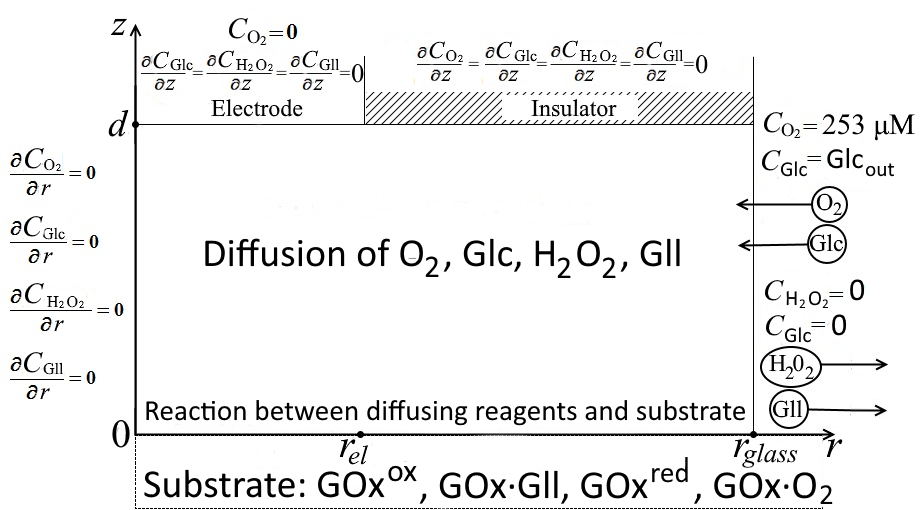
\includegraphics[width=1\linewidth]{chapter_1/Model_domain.png}
\caption{Scheme of simulation domain. All 8 reagents, boundary conditions for $C_{\text{diff}}$ and the direction of outside flux are displayed.}
\label{fig:Domain}
\end{figure}

Measurements of SECM acting in the redox-competition mode are changed into the scheme (\ref{fig:Domain}) due to the radial symmetry around the central axis of the electrode. Radial symmetry is a standard assumption in SECM modelling, though the case of off-centered UME was also investigated \cite{cornut2011accurate}.

According to the second Fick’s law \cite{laforge2008physicochemical}, diffusion processes are expressed by the system of partial differential equations (PDE):
\begin{equation}
  \begin{aligned}\label{eq:reakc_eq1}
  \frac{\partial C_{O_2}}{\partial t} &= D_{O_2}\,\Delta C_{O_2},\\
  \frac{\partial C_{Glc}}{\partial t} &= D_{Glc}\,\Delta C_{Glc},\\
  \frac{\partial C_{H_2 O_2}}{\partial t} &= D_{H_2 O_2} \,\Delta C_{H_2 O_2},\\
  \frac{\partial C_{Gll}}{\partial t} &= D_{Gll}\,\Delta C_{Gll},  \quad for\; 0<t\leq T,\; 0<z<d,\; 0<r<r_{glass},
  \end{aligned}
\end{equation}
where:
\begin{itemize}
  \item[] $C_{O_2}$, $C_{Glc}$, $C_{H_2 O_2}$ and $ C_{Gll}$ are concentrations of diffusing reagents and expressed as functions of time $t$ and spatial coordinates $z$ and $r$. Notation $C_{\text{diff}} = C_{\text{diff}} \left( t, z, r \right) = \left( C_{O_2}, C_{Glc}, \allowbreak C_{H_2 O_2}, \allowbreak C_{Gll} \right)$ was used when 4 diffusing re\-agents were considered together.
  \item[] $D_{O_2}$, $D_{Glc}$, $D_{H_2 O_2}$ and $D_{Gll}$ are diffusion coefficients of \ce{O2}, Glc, \ce{H2O2} and Gll.
  \item[] $d$ is the distance between the enzyme-modified surface and the electrode, which is varying from \SIrange{1}{120}{\um} as shown in Fig. \ref{fig:Domain}.
  \item[] $r_{glass} = \SI{80}{\um}$ is the radius of insulated area, $r_{el} = \SI{5}{\um}$ is the radius of electrode.
  \item[] $T$ is the duration of a computational experiment measured in seconds (the evaluation of this parameter is further explained in the next section).
  \item[] The Laplace operator $\Delta$ for concentration function $C$ in cylindrical coordinates with radial symmetry is
  \begin{equation*}
  \Delta C = \frac{1}{r}\frac{\partial }{\partial r} \left( r\frac{\partial C }{\partial r} \right) + \frac{\partial^{2} C}{\partial z^{2}}.
  \end{equation*}
\end{itemize}




% Please comment if you don't need to include and to compile latex manual
%%%%%%%%%%%%%%%%%%%%%%%%%%%%%%%%%%%%%%%%%%%%%%%%%%%%%%%%%%%%%%%%%%%%%%%%%%%%%%%%%%%%%%%%%%%%%%%%%%
%% Information about how to use latex
%% Most information is taken from University of Edinburgh Ph.D template 
%% https://www.overleaf.com/latex/templates/soe-thesis-template/dtfkrhyqjhqy

\chapter{\MakeUppercase{Template and short \LaTeX{} manual}} %Make it upper case to appear in TOC correctly
\label{cha:latex_manual}


This \LaTeX{} template and the instructions it contains will enable you to prepare your manuscript in an electronic format (pdf). 
Authors are responsible for ensuring the accuracy of all information contained in their manuscripts (e.g., proper names of organizations, data and findings, references, etc.).

\hologo{LaTeX} is a highly advanced type-setting system with a large number of various packages that can be loaded on demand to access certain type-setting functionalities.
Overleaf is a web service that enables you to write and type-set \LaTeX{} documents even more easily, as (1) it does not require you to install anything on your computer, (2) it saves your document securely online; and (3) it even implements version control so that you could return to some prior version of your document if really necessary.

It is not the intention of this template to list everything possible with \LaTeX. 
However, it will guide you for the most important type-setting issues you will definitely and/or most likely deal with.
You will see that, for many of them, we in fact direct you to online resources. This is because these are already of excellent quality and are continuously maintained. It also shows that, when it comes to \LaTeX{}, if you have a question, your best option to find the answer is to search online.


\section{Resources}
\label{sec:Resources}

We provide some explanations in the following sections on how to create and populate a \LaTeX{} document, 
but bear in mind that the following resources will soon come in handy.

\begin{description}
  \item[\href{https://learnxinyminutes.com/docs/latex}{LearnXinYminutes / LaTeX}]
    This gives a quick tour of \LaTeX{} (5 to 10 minutes).
    It is not meant to be a comprehensive, authoritative resource, but rather an overview of how it works and how to think about it.
    At the end of the tour it lists very useful resources.

  \item[\href{https://www.overleaf.com/learn}{Overleaf's documentation}]
    This template is hosted in Overleaf, an incredibly useful service for \LaTeX{}.
    The documentation is quite useful, and includes a 30-minute overview of \LaTeX{} as well as general introduction to key ideas.
  
  \item[\href{https://en.wikibooks.org/wiki/LaTeX}{WikiBook / LaTeX}]
    An amazing online guide to \LaTeX{}.
    It is well structured, comprehensive, and is easy to navigate.

  \item[\href{https://www.overleaf.com/gallery}{Overleaf's templates}]
    It is very common to have a look around and find other people's documents doing things that you might want to replicate in your document in terms of \LaTeX{} is used.
    For example, Overleaf includes a gallery that showcases things that might be helpful.

  \item[\href{https://tex.stackexchange.com/}{StackExchange / Tex}]
    Questions-Answers website for all things \LaTeX{}.
    Very often you can just literally write what you are trying to do
    and it will retrieve useful answers.
    In fact search engines often return StackExchange pages.

  \item[\href{https://ctan.org/}{CTAN}]
    CTAN is the Comprehensive TeX Archive Network.
    This is the main repository of all the packages that are available in \LaTeX{}.
    Packages tend to have great documentation.
    For example:
    \begin{description}
        \item[\href{https://ctan.org/pkg/hyperref}{hyperref}] 
            This is the package we use for cross-referencing and hyperlinks
            in this template.
        \item[\href{https://ctan.org/pkg/siunitx}{siunitx}]
            This package supports typesetting values with units.
    \end{description}
\end{description}



%%%%%%%%%%%%%%%%%%%%%%%%%%%%%%%%%%%%%%%%%%%%%%%%%%%%%%%%%%%%%%%%%%%%%%%%%%%%%%%%%%%%%%%%%%%
\section{File Structure}

Documents prepared and compiled with \LaTeX{} contain, in fact, a number of files.
The general principle is to dissociate content from formatting (aka typesetting) information | following a similar idea to web technology where HTML files normally contain content information while CSS files contain formatting information. The main file types are:

\begin{itemize}
  \item \verb|.tex| files: these files contain the content of your thesis. Not all the content has to be in one single file. It is totally fine to split it into multiple \verb|.tex| files, for example, one per chapter. In this case, one \verb|.tex| file acts as the main document and the other ones are called within it, using the function \verb|\include{...}|. In this template, the main document is the file \verb|thesis.tex|.
  % and, while most of the content is within it, the front matter content is in the \verb|frontmatter.tex| file which is included in \verb|thesis.tex|. Similarly, the acronyms and nomenclature entries are contained in the \verb|definitions.tex| file, and that file is called inside \verb|frontmatter.tex| (albeit with a different mechanism). More information about the front matter is found in \Cref{subsec:frontmatter}.
  Note that some typesetting information may be provided to \verb|.tex| files, but this should be for ad-hoc typesetting needs not covered in the other files described below.
  
  \item \verb|.sty| files: these files define what are called \emph{packages} that define typesetting. First, as you can see at the top of the \verb|thesis.tex| file, this thesis template uses the `book' \verb|documentclass|. That document class already comes with a number of pre-defined typesetting definitions. but, these can be altered or augmented with additional typesetting definitions by loading \emph{packages}. Packages come in two forms; they are either:           
    \begin{itemize}
        % \item Ad-hoc \verb|.sty| files that are added to your latex project. For example, this thesis template includes the \verb|UEDIN_SoE.ply| package; or
        \item Existing packages that can simply be loaded in \verb|.tex| or \verb|.ply|. Existing packages are loaded using the \verb|\usepackage{...}| function, and you can see at the beginning of the \verb|thesis.tex| file that this thesis template already loads a dozen packages. While we think these packages should already enable you to do most things you may wish to do in a thesis (e.g., add URLs or have figures with sub-figures), you may have additional needs. For this, simply search the resources listed in \Cref{sec:Resources}.
    \end{itemize}
  
  \item \verb|.bib| files: these are what are called Bibtex files. Bibtext is an open standard file format that is used to describe lists of references. This template document contains the \verb|thesis_bibliography.bib| file containing the references you wish to cite in the thesis. The file is called at the end of the \verb|thesis.tex| file (because the list of references goes at the end of the thesis), with the command \verb|\bibliography{thesis_bibliography}|.
  More information about how to add content to \verb|thesisReferences.bib| and cite those references in your thesis is provided in \Cref{sec:Bibligraphy}.
  
  \item Graphics/Image files: these are the graphics and images you wish to add to your thesis as figures. \hologo{LaTeX} supports many grapchics and image file formats, including: \verb|.png|, \verb|.jpeg| (\verb|.jpg|), \verb|.pdf| and \verb|.eps|. 
  You are most certainly familiar with the first three, but likely not the last one. 
  In fact, one should distinguish them into two groups:
      \begin{itemize}
        \item \emph{Raster formats} (\verb|.png| and \verb|.jpeg| (\verb|.jpg|)): these file formats store the graphic information as an array of pixels. This means that their file size grows with the number of pixels. These formats are recommended for storing photos/pictures or other types of graphics when the second group of formats below cannot be used or is not available. 
        
        \item \emph{Vector formats} (\verb|.eps| and \verb|.pdf|): these file formats store the graphic information in a vector format. For example, instead of storing a black line as a series of pixels, it will store it as a line object with a start and end point and black color. They also store text as the actual text. These formats are ideal for storing graphs, diagrams, and similar graphic objects. Note that using these formats normally lead to smaller file sizes (the image itself AND your final thesis), and they respond much better to graphic sizing in the template (e.g., adjusting text font size in accordance with the scaling of the image in the document). Importantly, note that if you take a graphic in raster format and save it in a vector format, it will not magically change the pixels into smart graphic objects. Any content in raster format will simply be re-included as raster content in the file. 
      \end{itemize}
      
      More information about how to generate vector graphic content and add figures to your document is provided in \Cref{sec:Figures}.
  
\end{itemize}



%%%%%%%%%%%%%%%%%%%%%%%%%%%%%%%%%%%%%%%%%%%%%%%%%%%%%%%%%%%%%%%%%%%%%%%%%%%%%%%%%%%%%%%%%%%
\section{Text Structure}
\label{sec:TextStructure}

The thesis comprises chapters that are composed of sections, sub-sections, etc.
To create such a heading structure, you can use the commands \verb|\chapter{}|, \verb|\section{}|, \verb|\subsection{}|, \verb|\subsubsection{}|, and \verb|\paragraph{}|. 
Note that, while \verb|\section{}| should be inside a \verb|\chapter{}|, a \verb|\subsection{}| inside a \verb|\section{}|, etc., a \verb|\paragraph{}| is not numbered and can thus be added inside any of those.

If you wish to cross-reference a heading elsewhere in the text, you will need to do two things. 
First, you must give that heading a \emph{label} using the command \verb|\label{}|, e.g., \verb|\label{sec:TextStructure}|. This label should be put right after the heading declaration: either on the same line or the next one.
Then, you can cross-reference the heading in the text using commands like \verb|\cref{}|.
More information about cross-referencing can be found in \Cref{sec:crossreferencing}.


% \subsection{Front matter}
% \label{subsec:frontmatter}

% The front matter of your thesis contains the title page and a number of sections, some mandatory, others optional. 
% In order, these are:
% \begin{description}
%     \item [Title page:] This is generated automatically by \LaTeX{}. To ensure it is complete, you must just enter your thesis title in the command \verb|\title{}| and your full name in the command \verb|\author{}|, both located at the beginning of the file \verb|thesis.tex|.
    
%     \item [Declaration:] This is generated automatically by \LaTeX{}. To ensure it is complete, you must just enter your full name in the command \verb|\author{}| (as already explained for the title page) and your supervisor's name in the command \verb|\supervisor{}|, both located at the beginning of the file \verb|thesis.tex|. The text content of the declaration is defined in the corresponding environment located in the file \verb|\frontmatter.tex|. However, you should not need to alter it. Also, note that the declaration page also adds your thesis word count automatically.
    
%     \item [Abstract:] This is mandatory. Your abstract should be in the region of 300 words long, containing 6 to 8 sentences covering the following:
%     \begin{enumerate}[noitemsep]
%         \item The scientific domain and the problem within the domain which is the subject matter of the thesis;
%         \item The research question to be answered in the thesis;
%         \item The means and methods (scientific tools) used to obtain the answer to the stated research question;
%         \item The answer to the research question; and
%         \item The meaning and importance of the answer and the results obtained,
%     \end{enumerate}
%     The text content of the abstract must be entered in the corresponding environment located in the file \verb|\frontmatter.tex|.
    
%     \item [Dedication:] This is optional, but commonly used by the students to thank various people for their support.  The text content of the dedication must be entered in the corresponding environment located in the file \verb|\frontmatter.tex|.
    
%     \item [Table of Content:] This is generated automatically by \LaTeX{}.
    
%     \item [List of Figures:] This is generated automatically by \LaTeX{}.
    
%     \item [List of Tables:] This is generated automatically by \LaTeX{}.
    
%     \item [Abbreviations:] This is required if you use abbreviations, in particular acronyms, in your thesis (which is very likely). All acronyms must be defined in the file \verb|definitions.tex|, as illustrated in it.
    
%     \item [Nomenclature:] This is optional but welcome if you use many mathematical variables throughout your thesis. All terms/variables must be defined in the file \verb|definitions.tex|, as illustrated in it. 
% \end{description}


\subsection{Lists}
\label{subsec:lists}

\begin{enumerate}
  \item Numbered lists should be presented using the environment \verb|enumerate| like in this example. 
  This environment applies the numbering and defines the format and spacing automatically. 
  \item Add the option \verb|[noitemsep]| to the environment to have no additional space between numbered list items (like is done here).
\end{enumerate}

\begin{itemize}
  \item Bulleted lists should be presented using the environment \verb|itemize| like in this example. 
  This environment applies the numbering and defines the format and spacing automatically. 
  \item Add the option \verb|[noitemsep]| to the environment to have no additional space between bulleted list items  (this is not done here).
\end{itemize}

\begin{description}
  \item[Label 1] Finally, description lists can be created when a label is preferred for each entry, as opposed to a bullet of a number.
  \item[Label 2] Add the option \verb|[noitemsep]| to the environment to have no additional space between bulleted list items (like is done here).
\end{description}
%
Note that the three lists above were generated using the environments and options described within them.
More information on how to create and format lists can be found at \url{https://www.overleaf.com/learn/latex/Lists}.



%%%%%%%%%%%%%%%%%%%%%%%%%%%%%%%%%%%%%%%%%%%%%%%%%%%%%%%%%%%%%%%%%%%%%%%%%%%%%%%%%%%%%%%%%%%
\section{Figures}
\label{sec:Figures}

%%%%%%%%%%%%%%%%%%%%%%%%%%%%%%%%%%%%%%%%%%%%%%%%%%%%%%%%%%%%%%%%%%%%
\subsection{Simple Figure}
\label{sec:SimpleFigure}

The lines below show an example of \LaTeX{} code to create an environment that displays the image \verb|graph_a.pdf|, gives it a caption and centres everything. 
It also gives the figure a label so that it can be easily cross-referenced in the text (see \Cref{sec:crossreferencing}. 
The figure produced by that code is shown as \Cref{fig:SimpleFigure}.

\begin{verbatim}
\begin{figure}[!ht]
  \centering
  \includegraphics[angle=-90,scale=0.4] %Rotates and scale
    {manual/images/graph_a.pdf}
  \caption{An example graph in PDF format.}
  \label{fig:SimpleFigure}
\end{figure}
\end{verbatim}

\begin{figure}[!ht]
  \centering
  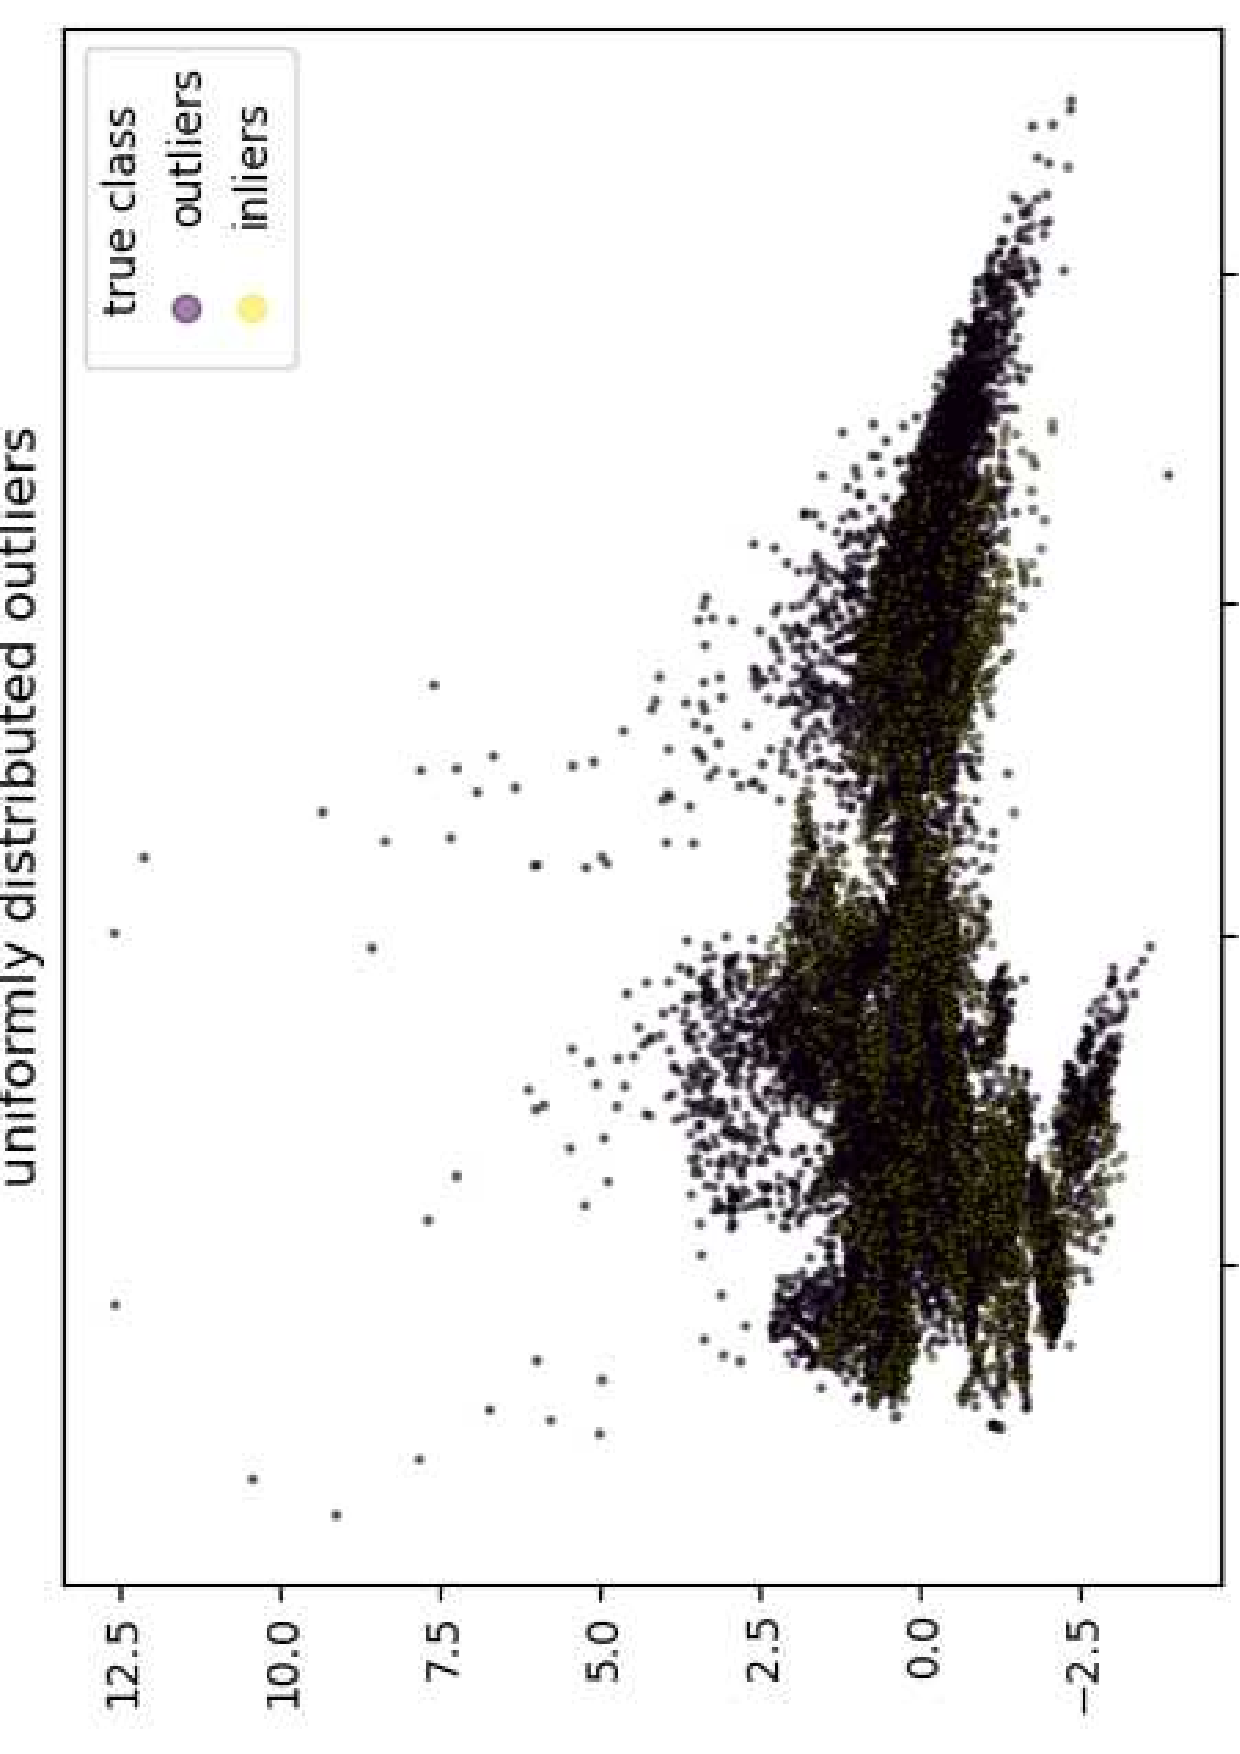
\includegraphics[angle=-90,scale=0.4]
    {manual/images/graph_a.pdf}
  \caption{An example graph in PDF format.}
  \label{fig:SimpleFigure}
\end{figure}

Note that you normally have to give the full path of an image in the \LaTeX{} project tree in order for it to be retrieved and loaded successfully.
We are recommending for each chapter folder create an  \emph{images} or  \emph{figures} folder and upload figures into this folder. Then, in the command \verb|includegraphics{}|, you need to give the full path to that image file. 
More information on creating and formatting figures can be found at \url{https://www.overleaf.com/learn/how-to/Including_images_on_Overleaf}.


%%%%%%%%%%%%%%%%%%%%%%%%%%%%%%%%%%%%%%%%%%%%%%%%%%%%%%%%%%%%%%%%%%%%
\subsection{Raster vs Vector format}
\label{sec:RasterVsVector}

\Cref{fig:RasterVsVector} shows what appears to be twice the same figure. However, the top one is rasterized (i.e., it is a grid of pixels) and is 83Kb in size, while the second is vectorized (i.e., canvas filled with shapes, including text) and is only 32Kb in size. 
The benefit of vectorized is not just the (generally) reduced size but also that it does not pixelate when zooming on it.

\begin{figure}[!ht]
    \centering
    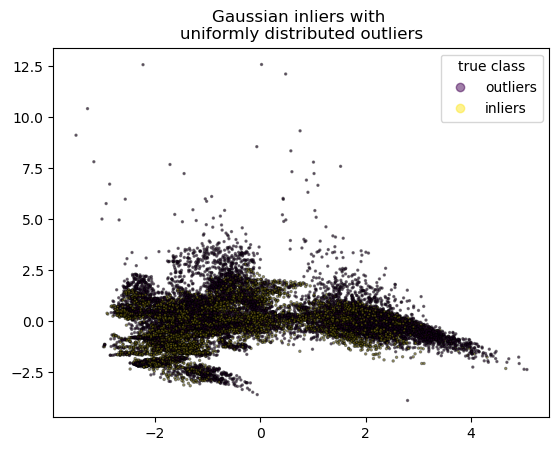
\includegraphics[width=0.8\textwidth]{manual/images/graph_a.png}
    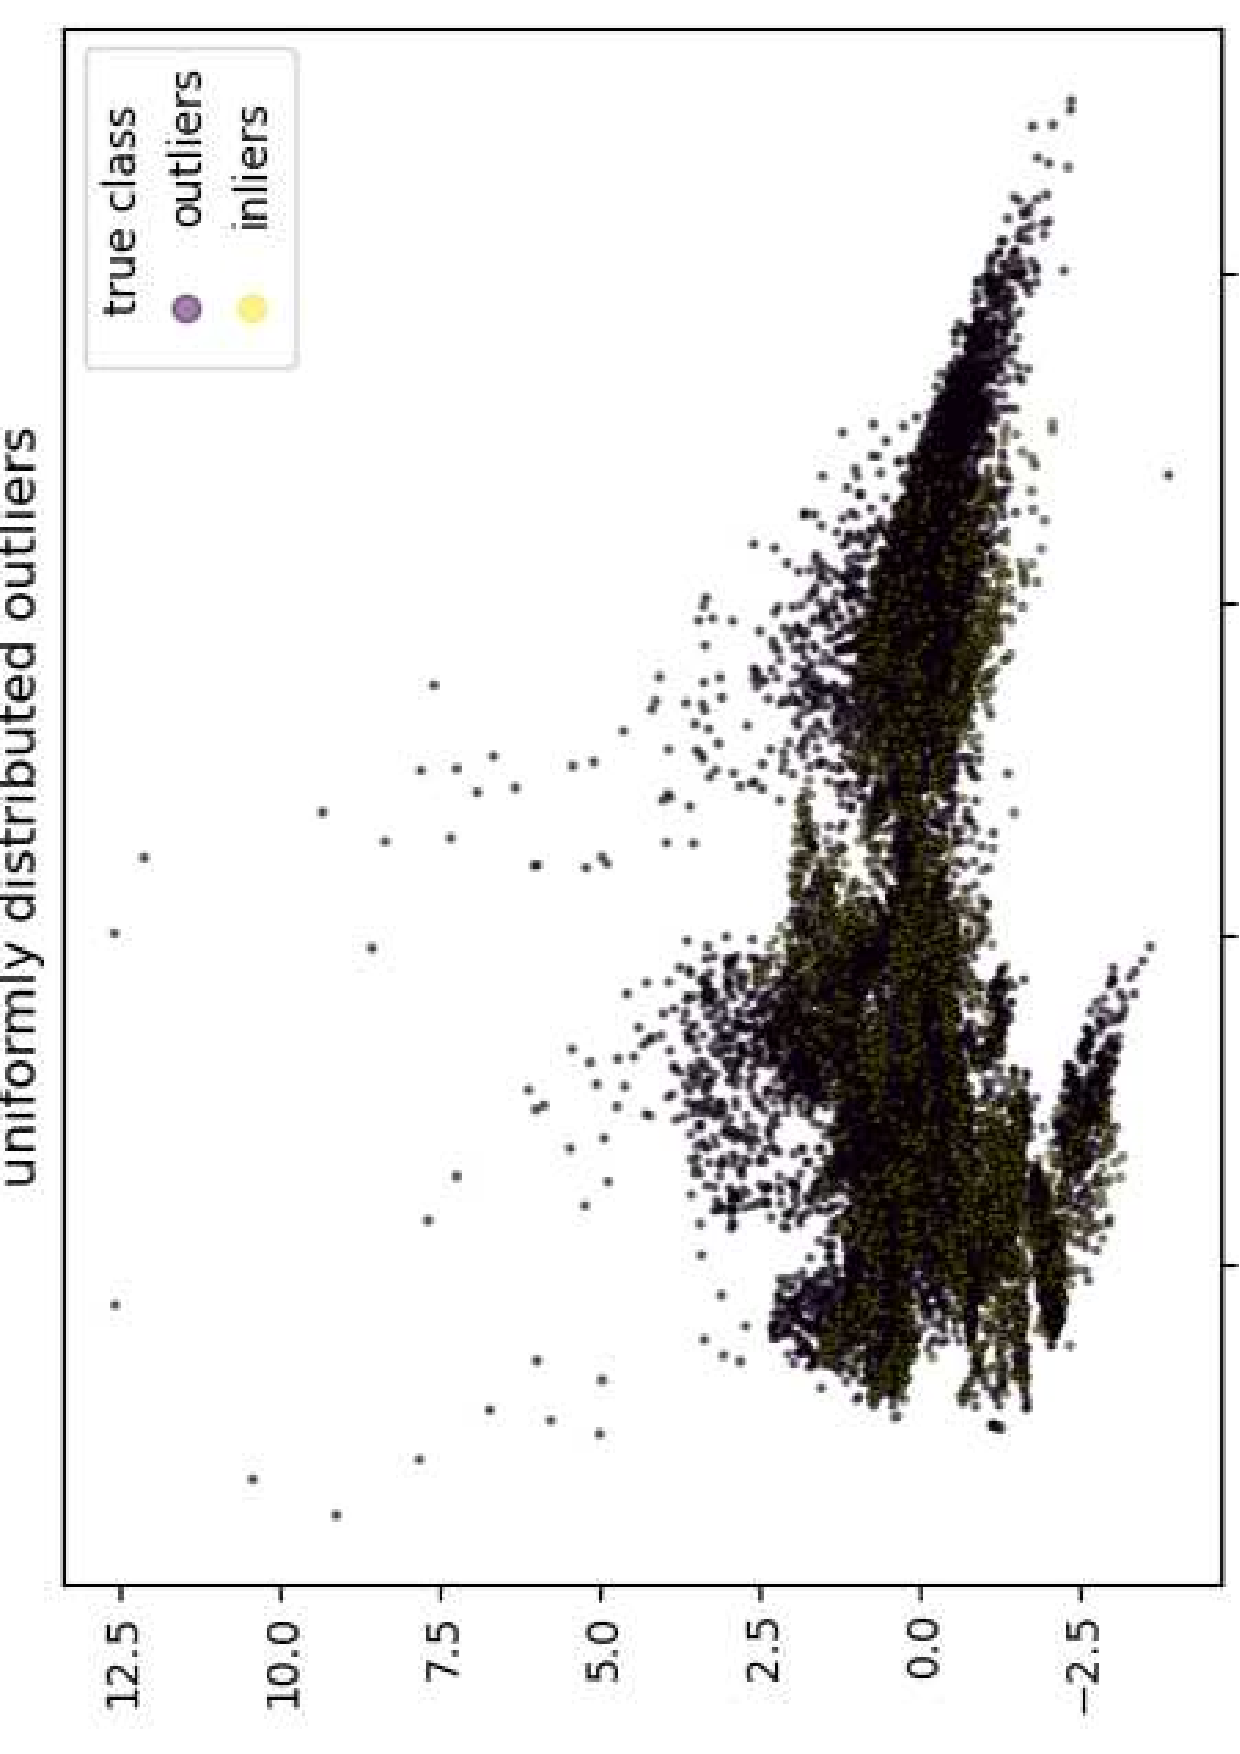
\includegraphics[angle=-90,width=0.8\textwidth]{manual/images/graph_a.pdf}
    \caption{My caption text}
    \label{fig:RasterVsVector}
\end{figure}

WARNING: ".eps" and ".pdf" are common formats used in LaTeX for vectorized images. However, having this file type does \textbf{not} necessarily mean that the content is vectorized.
For example, it is possible to save a ".png" picture of a graph into ".pdf". 
This does not magically transfer the picture into a vectorized image.

Useful software packages to create diagrams and vector images:
\begin{itemize}
    \item Draw.io (opensource): create diagrams (save EPS, or PDF)
    \item MS Powerpoint: create diagrams (save PDF)
    \item Inkscape (opensource): to manipulate vector file (e.g. crop PDF image from MS Powerpoint to fit content).
\end{itemize}


%%%%%%%%%%%%%%%%%%%%%%%%%%%%%%%%%%%%%%%%%%%%%%%%%%%%%%%%%%%%%%%%%%%%
\subsection{LaTeX-generated figure}
\label{sec:LaTeXFigure}

It is also possible to create diagrams in LaTeX using the package \verb|tikz| (which is already loaded for you in this template).
Here, only the data is supplied, and LaTeX code is used to create a diagram/figure layout and present the data content.
The advantage of this approach is that font and font sizing are set in coherence with that of the rest of the document.
However, it is quite tedious to create graphs/diagrams like that.

\Cref{fig:tikz} is an example of figure generated using the drawing package \verb|tikz|.

\begin{figure}
 \centering
 \begin{tikzpicture}
  \draw[step=1cm,gray,very thin] (0,0) grid (4,4);
  \draw[thick,->] (0,0) -- (4.5,0);
  \draw[thick,->] (0,0) -- (0,4.5);
  \foreach \x in {0,1,2,3,4}
   \draw (\x cm,1pt) -- (\x cm,-1pt) node[anchor=north] {$\x$};
  \foreach \y in {0,1,2,3,4}
   \draw (1pt,\y cm) -- (-1pt,\y cm) node[anchor=east] {$\y$};
   \draw[red,thick,dashed] (2,2) circle (1.5cm);
 \end{tikzpicture}
 \caption{A diagram generated using the TikZ package.}
 \label{fig:tikz}
\end{figure}


%%%%%%%%%%%%%%%%%%%%%%%%%%%%%%%%%%%%%%%%%%%%%%%%%%%%%%%%%%%%%%%%%%%%
\subsection{Sub-figures}
\label{sec:SubFigures}

It is possible to create figures with subfigures. 
This requires the use of the packages \verb|caption| and \verb|subcaption| (which are already loaded for you in this template).

Usage is shown in \Cref{fig:Subfigures}. 
You can see both subfigures have labels, which means you can cross-reference them individually in the text as \Cref{fig:Subfigure1} and \Cref{fig:Subfigure2} (see \Cref{sec:crossreferencing} for details on cross-referencing).
More details on how to create a figure with subfigures can be found at \url{https://www.overleaf.com/learn/latex/How_to_Write_a_Thesis_in_LaTeX_(Part_3)\%3A_Figures\%2C_Subfigures_and_Tables}.


\begin{figure}[!ht]
     \centering
     \begin{subfigure}[b]{0.45\textwidth}
         \centering
         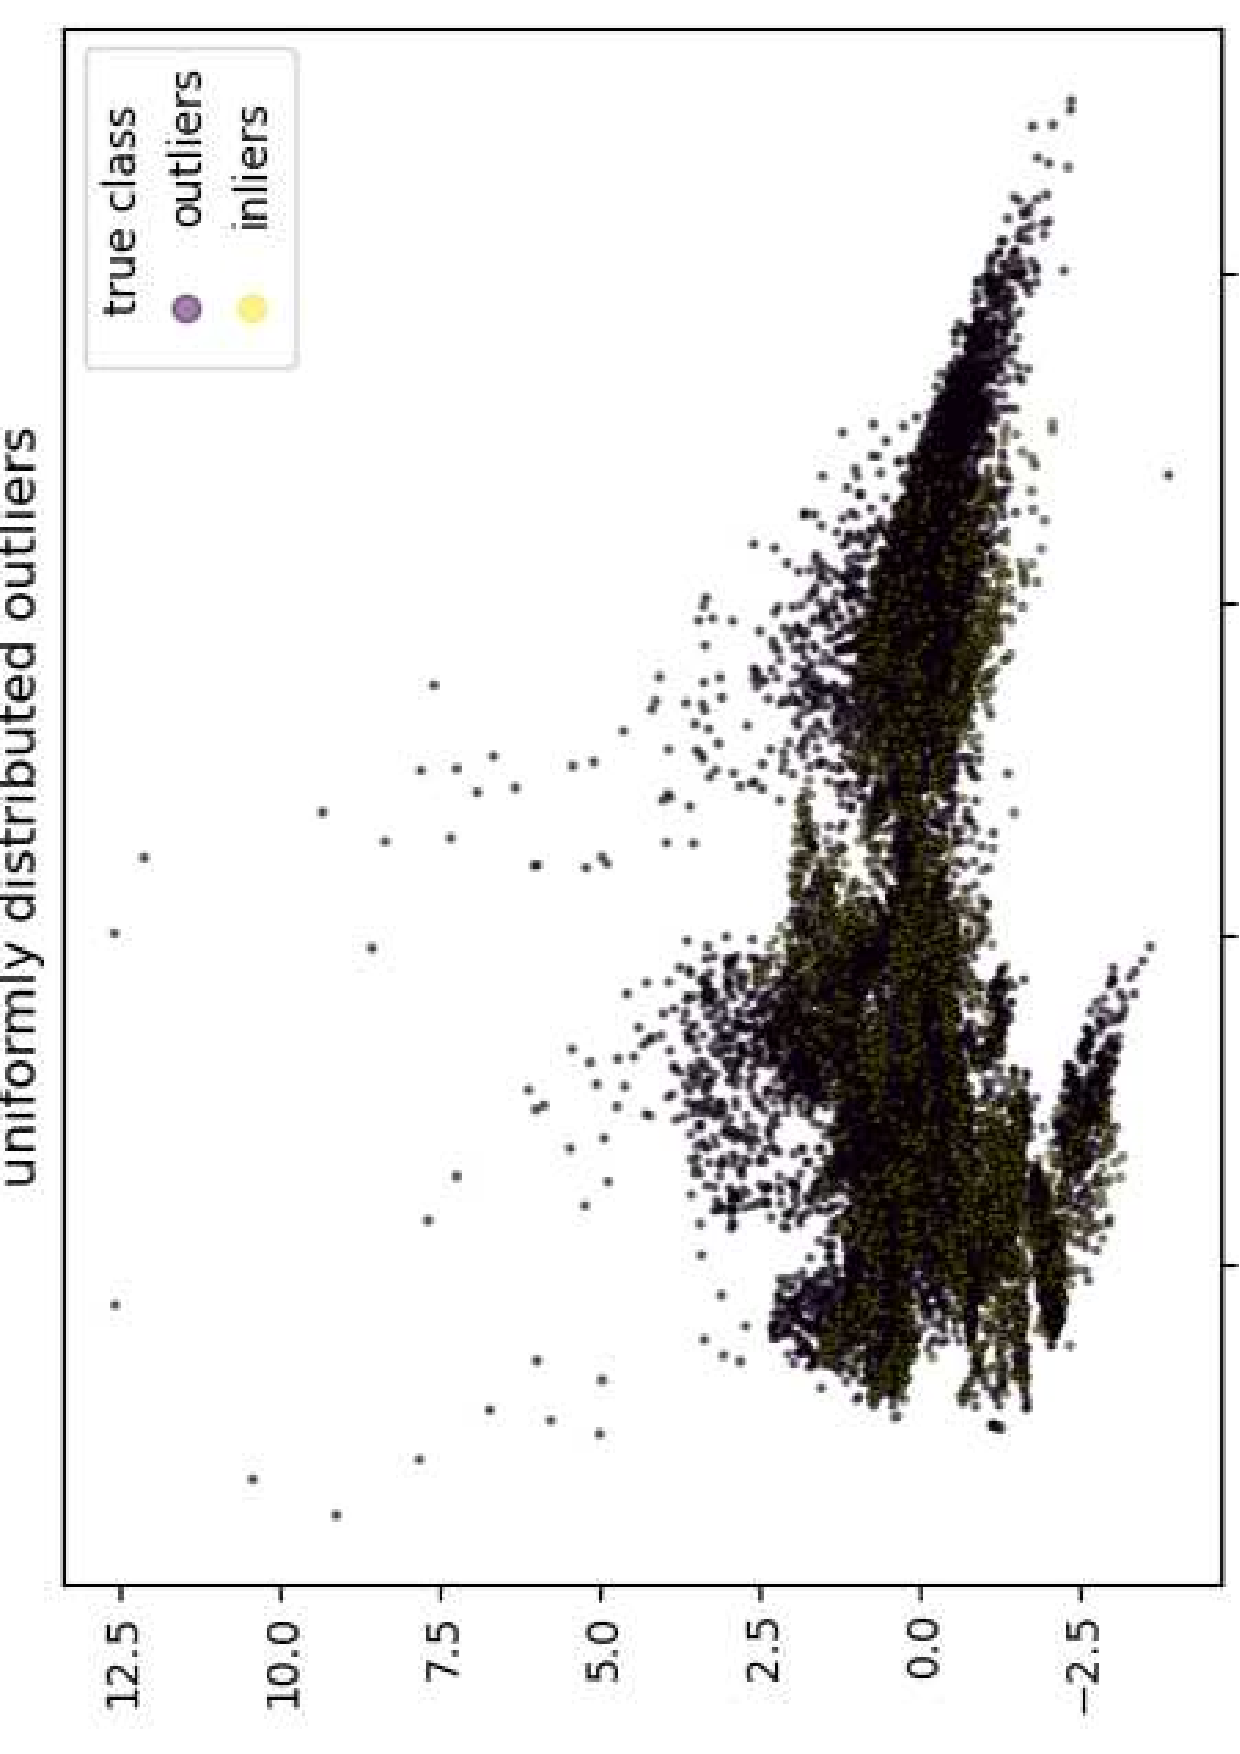
\includegraphics[angle=-90,width=\textwidth]{manual/images/graph_a.pdf}
         \caption{Caption of subfigure 1}
         \label{fig:Subfigure1}
     \end{subfigure}
     \hfill
     \begin{subfigure}[b]{0.45\textwidth}
         \centering
         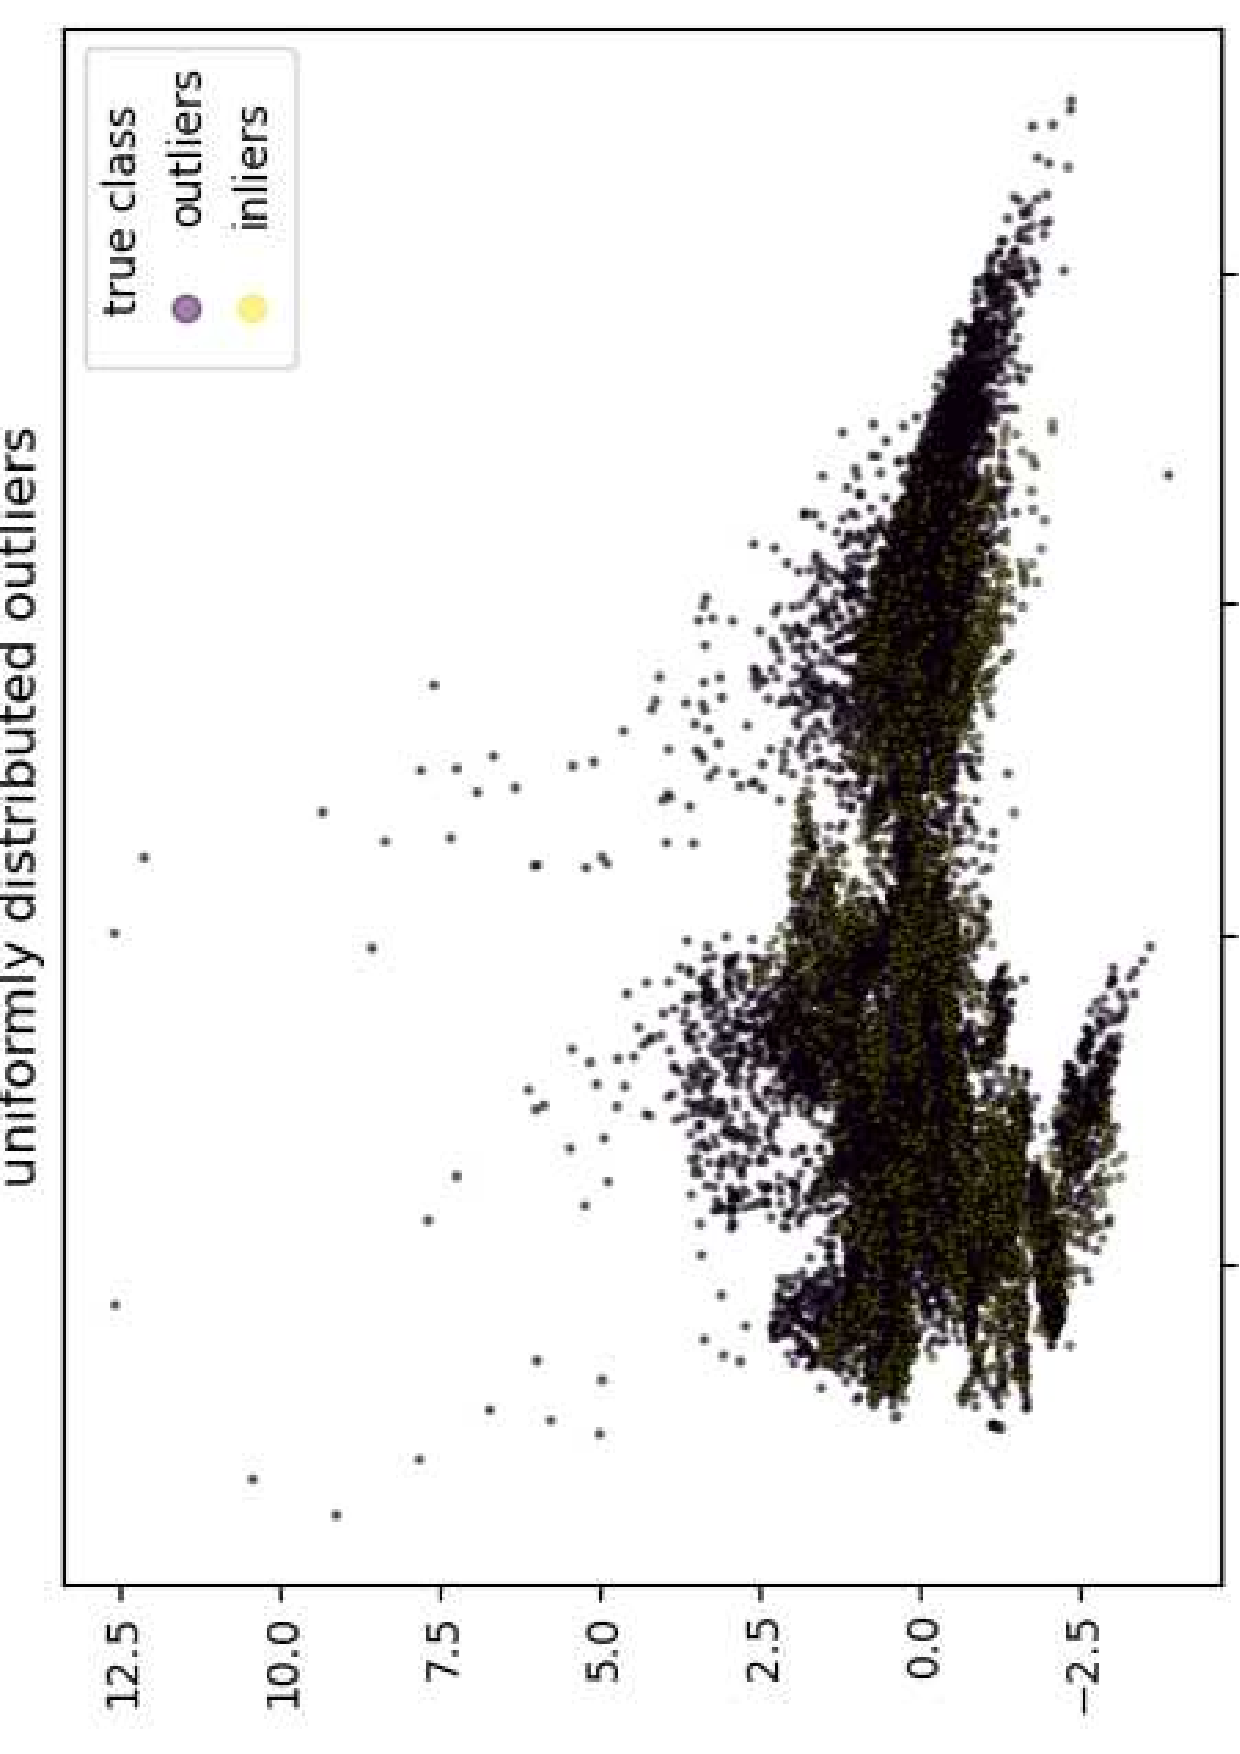
\includegraphics[angle=-90,width=\textwidth]{manual/images/graph_a.pdf}
         \caption{Caption of subfigure 2}
         \label{fig:Subfigure2}
     \end{subfigure}
     \caption{Caption of overall figure}
     \label{fig:Subfigures}
\end{figure}


%%%%%%%%%%%%%%%%%%%%%%
\subsection{And more...}
\label{sec:FiguresMore}

Many other formatting/typesetting options exist. 
For example, you can put a figure in landscape mode using the environment \verb|sidewayfigure| provided by the package \verb|rotating|.

More information on how to create and format figures can be found at \url{https://www.overleaf.com/learn/latex/Inserting_Images}.
But, once again, if you have any specific need, we recommend you search for solutions at the locations suggested in \Cref{sec:Resources} or by using your favorite search engine.



%%%%%%%%%%%%%%%%%%%%%%%%%%%%%%%%%%%%%%%%%%%%%%%%%%%%%%%%%%%%%%%%%%%%%%%%%%%%%%%%%%%%%%%%%%%
\section{Tables}
\label{sec:Tables}

%%%%%%%%%%%%%%%%%%%%%%%%%%%%%%%%%%%%%%%%%%%%%%%%%%%%%%%%%%%%%%%%%%%%
\subsection{Simple Table}
\label{sec:SimpleTable}

The lines below show an example of \LaTeX{} code to create an environment that defines a table \verb|graph_a.pdf|, gives it a caption, and centers everything.
It also gives the table a label so that it can be easily cross-referenced in the text. The table produced by that code is also shown as \Cref{tab:MyFirstTable}.

\begin{verbatim}
\begin{table}[!ht]
    \centering
    \begin{tabular}{|c c c c|} 
    \hline
    Col1 & Col2 & Col2 & Col3 \\
    \hline
    1 & 6 & 87837 & 787 \\ 
    2 & 7 & 78 & 5415 \\
    3 & 545 & 778 & 7507 \\
    4 & 545 & 18744 & 7560 \\
    5 & 88 & 788 & 6344 \\
    \hline
    \end{tabular}
    \caption{Table to test captions and labels.}
    \label{tab:MyFirstTable}
\end{table}
\end{verbatim}

\begin{table}[!ht]
    \centering
    \begin{tabular}{|c c c c|} 
    \hline
    Col1 & Col2 & Col2 & Col3 \\
    \hline
    1 & 6 & 87837 & 787 \\ 
    2 & 7 & 78 & 5415 \\
    3 & 545 & 778 & 7507 \\
    4 & 545 & 18744 & 7560 \\
    5 & 88 & 788 & 6344 \\
    \hline
    \end{tabular}
    \caption{Table to test captions and labels.}
    \label{tab:MyFirstTable}
\end{table}

In this code, the \emph{table} environment (i.e. \verb|\begin{table}...\end{table}|) creates a floating environment of the type 'table' that can be given a caption and a label. 
\verb|\centering| centers the table inside that table floating environment. 
Then, the \emph{tabular} environment is the environment that contains the description of the table. 
The tabular environment argument tells \LaTeX{} the alignment to be used in each column and the vertical lines to insert. 
In the table above, \verb!|c c c c|! defines a table with four columns in all of which the text is centered. 
Inside the \emph{tabular} environment, \verb|\hline| creates a horizontal line through the table (you can use the command \verb|\cline{...}| to make a horizontal line that only spans a subset of the columns). Finally, each row of data is entered with the cell content delimited with the character \verb|&| and the end of the row marked with the characters \verb|\\|.


%%%%%%%%%%%%%%%%%%%%%%%%%%%%%%%%%%%%%%%%%%%%%%%%%%%%%%%%%%%%%%%%%%%%
\subsection{Merging Rows and Columns}
\label{sec:TableRowMerging}

If you wish to merge some cells together horizontally or vertically, use the \verb|\multicolumn{...}|) or \verb|\multirow{...}| commands, the latter requiring the \verb|multirow| package (which already loaded for you in this template).
\Cref{tab:MySecondTable} shows an example of table containing both merges columns and merged cells.

\begin{table}[!ht]
    \centering
    \caption{Table with merged cells.}
    \label{tab:MySecondTable}
    \begin{tabular}{|cccc|} 
    \hline
    Col1 & Col2 & Col2 & Col3 \\
    \hline
    \multicolumn{2}{|c}{7} & 87837 & 787 \\  
    \multirow{2}{*}{5} & 7 & 78 & 5415 \\ 
    & 545 & 778 & 7507 \\
    4 & 545 & 18744 & 7560 \\
    5 & 88 & 788 & 6344 \\
 \hline
 \end{tabular}
\end{table}

If you have to insert a very long table, which takes up two or more pages in your document, use the \emph{longtable} package (already loaded for you in this template). If you wish to have your table in landscape mode, consider using the \emph{sidewaystable} or \emph{landscape} packages.  

More information on how to create and format tables (including how to color rows/cells) can be found at \url{https://www.overleaf.com/learn/latex/Tables} and many other places at the resources listed in \Cref{sec:Resources} and elsewhere on the web.




%%%%%%%%%%%%%%%%%%%%%%%%%%%%%%%%%%%%%%%%%%%%%%%%%%%%%%%%%%%%%%%%%%%%
\subsection{Column Widths}
\label{sec:TableColumnWidths}

As mentioned, in the tables above, \verb!|c c c c|! defines a table with four columns in all of which the text is centered (it also instructs that double vertical lines should bind the table on the left and right).
However, as illustrated in \Cref{tab:MyThirdTable1}, the width of each column expands in order to accommodate the largest width of the content of any of its cells; there is no text wrapping.

To address this, you can replace the first \verb|c| with \verb|p{0.2\textwidth}| which forces the first column to have a width of no more than $20\%$ of the text width, which triggers some text wrapping in this case.
This approach is illustrated with the first column of \Cref{tab:MyThirdTable}.
However, note that the content of the cells in that column is not centred anymore. 
To retain text centering, \verb|p{0.2\textwidth}| needs to be prepended by \verb|>{\centering}|, which is illustrated for the second column of \Cref{tab:MyThirdTable}.

\begin{table}[!ht]
    \centering
    \caption{Table with fixed column widths.}
    \label{tab:MyThirdTable1}
    \begin{tabular}{|c c c c|} 
    \hline
    Col1 & Col2 & Col2 & Col3 \\
    \hline
    1 & 6 & 87837 & 787 \\  
    Best table in the world & 7 & 78 & 5415 \\ 
    3 & 545 & 778 & 7507 \\
    4 & 545 & 18744 & 7560 \\
    5 & 88 & 788 & 6344 \\
    \hline
    \end{tabular}
\end{table}

\begin{table}[!ht]
    \centering
    \caption{Table with fixed column widths.}
    \label{tab:MyThirdTable}
    \begin{tabular}{|p{0.2\textwidth}>{\centering}p{0.2\textwidth}cc|} 
    \hline
    Col1 & Col2 & Col2 & Col3 \\
    \hline
    1 & 6 & 87837 & 787 \\  
    Best table in the world & 7 & 78 & 5415 \\ 
    3 & 545 & 778 & 7507 \\
    4 & 545 & 18744 & 7560 \\
    5 & 88 & 788 & 6344 \\
    \hline
    \end{tabular}
\end{table}





%%%%%%%%%%%%%%%%%%%%%%%%%%%%%%%%%%%%%%%%%%%%%%%%%%%%%%%%%%%%%%%%%%%%
\subsection{Colouring Cells}
\label{sec:TableColouring}

You may wish to color cells in a table you created.
This can be done by loading the package \verb|xcolor| (already loaded for you in this template), and using the \verb|cellcolor{...}| command in the cell to be coloured.
This is illustrated in \Cref{tab:MyFourthTable}.

It is also possible to color an entire column at once.
This requires defining a new column type.
\Cref{tab:MyFifthTable} illustrates this with the new column type \verb|G| define in the preamble of this \LaTeX{} document as:

\begin{verbatim}
\newcolumntype{G}{>{\centering\columncolor{blue!20!white}}p{0.2\textwidth}}
\end{verbatim}


\begin{table}[!ht]
    \centering
    \caption{Table with coloured cell.}
    \label{tab:MyFourthTable}
    \begin{tabular}{|cccc|} 
    \hline
    Col1 & Col2 & Col2 & Col3 \\
    \hline
    1 & 6 & 87837 & 787 \\  
    2 & \cellcolor{blue} 7 & 78 & 5415 \\ 
    3 & 545 & 778 & 7507 \\
    4 & 545 & 18744 & 7560 \\
    5 & 88 & 788 & 6344 \\
    \hline
    \end{tabular}
\end{table}

%Define this command in preamble to use it in whole document
\newcolumntype{G}{>{\centering\columncolor{blue!20!white}}p{0.2\textwidth}}
\begin{table}[!ht]
    \centering
    \caption{Table with coloured column.}
    \label{tab:MyFifthTable}
    \begin{tabular}{||cGcc||} 
    \hline
    Col1 & Col2 & Col2 & Col3 \\
    \hline\hline
    1 & 6 & 87837 & 787 \\  
    2 & 7 & 78 & 5415 \\ 
    3 & 545 & 778 & 7507 \\
    4 & 545 & 18744 & 7560 \\
    5 & 88 & 788 & 6344 \\
 \hline
 \end{tabular}
\end{table}



%%%%%%%%%%%%%%%%%%%%%%%%%%%%%%%%%%%%%%%%%%%%%%%%%%%%%%%%%%%%%%%%%%%%
\subsection{Multipage Table}
\label{sec:TableMultipage}

When typesetting a table, you may come across a table whose content makes it span more than a page. 
\LaTeX{} does not handle these situations, by splitting the table automatically across two (or more) pages.
Instead, you have to change your table environment to a \verb|longtable| environment and provide the necessary information whether and how to repeat the table caption on each page, repeat the column headers, etc. 
How this is achieved is illustrated with \Cref{tab:TableLong}.


\begin{longtable}{|l|l|l|}
    \caption{A sample long table.} 
    \label{tab:TableLong} \\
    
    \hline 
    \textbf{First column} & \textbf{Second column} & \textbf{Third column} \\ 
    \hline 
    \endfirsthead
    
    \multicolumn{3}{c}{{\tablename\ \thetable{} -- continued from previous page}} \\
    \hline 
    \textbf{First column} & \textbf{Second column} & \textbf{Third column} \\ 
    \hline 
    \endhead
    
    
    \hline \multicolumn{3}{|r|}{{Continued on next page}} \\ \hline
    \endfoot
    
    \hline \hline
    \endlastfoot

One & abcdef ghjijklmn & 123.456778 \\
One & abcdef ghjijklmn & 123.456778 \\
One & abcdef ghjijklmn & 123.456778 \\
One & abcdef ghjijklmn & 123.456778 \\
One & abcdef ghjijklmn & 123.456778 \\
One & abcdef ghjijklmn & 123.456778 \\
One & abcdef ghjijklmn & 123.456778 \\
One & abcdef ghjijklmn & 123.456778 \\
One & abcdef ghjijklmn & 123.456778 \\
One & abcdef ghjijklmn & 123.456778 \\
One & abcdef ghjijklmn & 123.456778 \\
One & abcdef ghjijklmn & 123.456778 \\
One & abcdef ghjijklmn & 123.456778 \\
One & abcdef ghjijklmn & 123.456778 \\
One & abcdef ghjijklmn & 123.456778 \\
One & abcdef ghjijklmn & 123.456778 \\
One & abcdef ghjijklmn & 123.456778 \\
One & abcdef ghjijklmn & 123.456778 \\
One & abcdef ghjijklmn & 123.456778 \\
One & abcdef ghjijklmn & 123.456778 \\
One & abcdef ghjijklmn & 123.456778 \\
One & abcdef ghjijklmn & 123.456778 \\
One & abcdef ghjijklmn & 123.456778 \\
One & abcdef ghjijklmn & 123.456778 \\
One & abcdef ghjijklmn & 123.456778 \\
One & abcdef ghjijklmn & 123.456778 \\
One & abcdef ghjijklmn & 123.456778 \\
One & abcdef ghjijklmn & 123.456778 \\
\end{longtable}





%%%%%%%%%%%%%%%%%%%%%%%%%%%%%%%%%%%%%%%%%%%%%%%%%%%%%%%%%%%%%%%%%%%%%%%%%%%%%%%%%%%%%%%%%%%
\section{Mathematical Expressions}
\label{sec:Math}

%%%%%%%%%%%%%%%%%%%%%%%%%%%%%%%%%%%%%%%%%%%%%%%%%%%%%%%%%%%%%%%%%%%%%%%%%%%%%%%
\subsection{Inline vs Display Mode}
\label{sec:MathModes}

Mathematical expressions, including formulas, can be entered in two different ways: \emph{inline} mode or \emph{display} mode. 
Inline mode means that the mathematical expression will appear within the text; display mode means that it will appear in a separate line (or set of lines).

You can use two types of delimiters to typeset mathematical expressions in inline mode, \verb|\(...\)| or \verb|$...$|, or the \emph{math} environment \verb|\begin{math}...\end{math}|. 
Two examples of inline mathematical expressions are \(d=\sqrt{x^2+y^2}\) and $M = A + B$.

You can use the delimiters \verb|\[...\]| or the \emph{displaymath} \emph{equation} or \emph{align} environments \verb|\begin{equation}| \verb|...\end{equation}| to typeset mathematical expressions in display mode.

An example of mathematical expression in display mode is: \[d=\sqrt{x^2+y^2}\]

An example of mathematical expression in display mode is: \begin{displaymath}d=\sqrt{x^2+y^2}\end{displaymath}

An example of mathematical expression in display mode is: \begin{equation}d=\sqrt{x^2+y^2}\end{equation}



%%%%%%%%%%%%%%%%%%%%%%%%%%%%%%%%%%%%%%%%%%%%%%%%%%%%%%%%%%%%%%%%%%%%
\subsection{Mathematical Symbols and Greek letters}
\label{sec:MathSymbols}

You can use an extremely broad range of Greek letters and mathematical symbols, such as:
\begin{itemize}[nosep]
  \item Binary operators: $\times \otimes \oplus \cup \cap$ 
  \item Relation operators: $< > \subset \supset \subseteq \supseteq$
  \item Greek letters: $\alpha \beta \gamma \rho \sigma \delta \epsilon$, and $A B \Gamma \Sigma \Delta E$
  \item Other: $\int \oint \sum \prod$
\end{itemize}
%
A first list of mathematical symbols can be found at \url{https://www.overleaf.com/learn/latex/List_of_Greek_letters_and_math_symbols} with an even more detailed list of symbols available at \url{https://oeis.org/wiki/List_of_LaTeX_mathematical_symbols}.


%%%%%%%%%%%%%%%%%%%%%%%%%%%%%%%%%%%%%%%%%%%%%%%%%%%%%%%%%%%%%%%%%%%%
\subsection{Equation}
\label{sec:MathEquations}

\LaTeX{} is extremely powerful in general, but in particular when it comes to typesetting mathematical expressions, such as equations. 
The equation below is just one example. 
As you can see, 

\begin{align}\label{eq:MyEquation}
\begin{split}
S(\omega) 
&= \frac{\alpha g^2}{\omega^5} e^{[ -0.74\bigl\{\frac{\omega U_\omega 19.5}{g}\bigr\}^{\!-4}\,]} \\
&= \frac{\alpha g^2}{\omega^5} \exp\Bigl[ -0.74\Bigl\{\frac{\omega U_\omega 19.5}{g}\Bigr\}^{\!-4}\,\Bigr] 
\end{split}
\end{align}


%%%%%%%%%%%%%%%%%%%%%%
\subsection{And more...}
\label{sec:MathMore}

Further details about typesetting mathematical expressions can be found at \url{https://www.overleaf.com/learn/latex/Mathematical_expressions}.




%%%%%%%%%%%%%%%%%%%%%%%%%%%%%%%%%%%%%%%%%%%%%%%%%%%%%%%%%%%%%%%%%%%%%%%%%%%%%%%%%%%%%%%%%%%
\section{Properly Typesetting Units}

In any scientific and engineering piece of work units play a major part. Without them our numerical information is practically useless. We need to be able to properly typeset them as in publishing, they often do follow specific rules that, sadly, most of the time, simple word processing packages ignore. Units, for example, are not set in italics or in random fonts that we seem to be using.

There are many \LaTeX{} packages you can use and explore to help you typeset units properly, but in this template, we use the \verb|siunitx| package. 

For example, \verb|\unit{kg.m.s^{-1}}| produces \unit{kg.m.s^{-1}}. \\
\verb|\unit{\kilogram\metre\per\second}| produces the same output \unit{\kilogram\metre\per\second}.

If you want to nicely refer to an angle you can just type \verb|\ang{10}| to get \ang{10} or \verb|\ang{3;23;5}| for \ang{3;23;5} or type \verb|\qty{3}{mm}| for \qty{3}{mm} or more explicitly \verb|\qty{3}{\milli\metre}| for the same effect as \qty{3}{\milli\metre}. 
\verb|\qtylist{5;10;15}{\metre}| will produce nicely \qtylist{5;10;15}{\metre}. 
\verb|\qtyproduct{5 x 10 x 15}{\metre}| produces \qtyproduct{5 x 10 x 15}{\metre}.


The options are very comprehensive, and no matter how complex or simple your units are they will be typeset properly and beautifully.
Detailed instructions on how to use the various commands that the \verb|siunitx| package makes available for typesetting units properly are given in \url{https://mirror-hk.koddos.net/CTAN/macros/latex/contrib/siunitx/siunitx.pdf}



%%%%%%%%%%%%%%%%%%%%%%%%%%%%%%%%%%%%%%%%%%%%%%%%%%%%%%%%%%%%%%%%%%%%%%%%%%%%%%%%%%%%%%%%%%%
\section{Cross-referencing}
\label{sec:crossreferencing}

Your work will have internal references to various objects like equations, figures, chapters, sections, etc. Let's have a look at some examples.

Using the readily available command \verb|\ref{}|, you can automatically reference such objects. For example:
\begin{itemize}
    \item \verb|Section~\ref{sec:Figures}| typesets `Section~\ref{sec:Figures}'
    \item \verb|Figure~\ref{fig:SimpleFigure}| typesets `Figure~\ref{fig:SimpleFigure}'
    \item \verb|Table~\ref{tab:MyFirstTable}| typesets `Table~\ref{tab:MyFirstTable}'
    \item \verb|Equation \ref{eq:sedov}| typesets `Equation \ref{eq:MyEquation}'
\end{itemize}

However, \verb|\ref{}| requires you to actually type the type of object referenced, i.e.,  \verb|Section| in \verb|Section~\ref{sec:Figures}| in order to obtain `Section~\ref{sec:Figures}'. 
A smart and easier way to cross-reference is to use the \verb|cleveref| package (already loaded for you in this template).
The \verb|cleveref| package provides the commands \verb|\cref{}|, \verb|\Cref{}|, \verb|\crefrange{}|, and many more. For example:
\begin{itemize}
    \item \verb|\cref{sec:Figures}| typesets `\cref{sec:Figures}' and \verb|\cref{tab:MyFirstTable}| typesets `\cref{tab:MyFirstTable}'
    \item \verb|\Cref{sec:Figures}| typesets `\Cref{sec:Figures}'
    \item \verb|\cref{sec:Figures,sec:Math}| typesets `\cref{sec:Figures,sec:Math}'
    \item \verb|\crefrange{sec:Figures}{sec:Math}| typesets `\crefrange{sec:Figures}{sec:Math}'
\end{itemize}
%
These commands automatically identify the type of each referenced object and ensure that those types are typeset consistently throughout the document.

Although \LaTeX{} does not require it, it is good practice to try and name labels by giving an indication of what they represent, such as \verb|\label{sec:...}| for labels of sections and sub-sections.
This way, they can be retrieved easily and not be confused.




%%%%%%%%%%%%%%%%%%%%%%%%%%%%%%%%%%%%%%%%%%%%%%%%%%%%%%%%%%%%%%%%%%%%%%%%%%%%%%%%%%%%%%%%%%%
\section{Bibliography and Citations}
\label{sec:Bibligraphy}

Citations of works that support your arguments and are used to reference and acknowledge the original sources of information that you use, discuss, or develop are very easy. 

\LaTeX{} uses a specific methodology to describe and process lists of references: Bibtex (\url{http://www.bibtex.org}).
Bibtex manifest itself in your \LaTeX{} project in the form of a file with extension \verb|.bib| and requires loading the package \verb|natbib| to be able to process \verb|.bib| files and typeset the information they contain.
In the current project, the file is called \verb|thesis_bibliography.bib|.
The file has a simple text format and essentially contains a database of entries.
The most common entry is for an \verb|@article|, but there are many more, as can be seen in the example file \verb|thesis_bibliography.bib|. 
What is important is that every entry you create has its own unique label that is then used to \emph{cite} the entry appropriately in your \LaTeX{} text and create the list of references that is created automatically and included at the end of our thesis.

Citations in the text are made using the commands \verb|\citet| and \verb|\citep| and possibly \verb|\citeauthor| or other forms of citation commands useful for more specific cases.
For example, "\citet{demoArticle} provided a comprehensive survey in their review paper" is obtained using the command \verb|\citet{demoArticle}|.
This command creates an entry that has the authors names as part of the sentence (here used as subjects). 
In contrast, "a comprehensive survey is provided in \citep{demoArticle}" is obtained using the command \verb|\citep{demoArticle}|. 
This commands just creates an entry that is just citation to the reference.
Also note that an entry in the list of references, located at the end of the thesis.

You must let \LaTeX{} know where the bib file is that contains the details of the references that you cite in you \verb|tex| file.
This is done by adding the command \verb|\bibliography{file.bib}| in your main \verb|.tex| file.
In this thesis template, \verb|\bibliography{thesis_bibliography.bib}| is added at the end of the \verb|bibiography/bibliography.tex| file.

\LaTeX{}, in combination with its bibliography packages, can create any style of referencing that you might need and more information can be found at  \url{https://www.overleaf.com/learn/latex/Bibliography_management_with_natbib} or using different packages \url{https://www.overleaf.com/learn/latex/Bibliography_management_with_bibtex} or alternatively \url{https://www.overleaf.com/learn/latex/Bibliography_management_with_biblatex}.
% However, for this thesis template, we have already selected the AGSM style (and suggest you keep it) that is defined in the \verb|thesis.tex| file with the command \verb|\bibliographystyle{agsm}|.
However, for this thesis template, we have already selected the abbrvnat style (and suggest you keep it) that is defined in the \verb|/bibiography/bibliography.tex| file with the command \verb|\bibliographystyle{abbrvnat}|.

\textbf{Note:} An emerging alternative to the use of \emph{Bibtex} (used with the \verb|natbib| package) is emerging.
It is called \emph{Biber} (used with the \verb|biblatex| package).
We do not explain here how to work with Biber, but it is, in fact, very similar to working with Bibtex. 
For now, we, however, recommend sticking to Bibtex.

%%%%%%%%%%%%%%%%%%%%%%%%%%%%%%%%%%%%%%%%%%%%%%%%%%%%%%%%%%%%%%%%%%%%%%%%%%%%%%%%%%%%%%%%%%%
\section{Glossary}
\label{sec:Glossary}

A glossary\index{Glossary} is a specialized list of terms and definitions often found at the end of a book, article, 
or in a field of study. It is an alphabetical list of words pertaining to a specific subject, with explanations; 
a reference tool to aid understanding of specialized language. 
You can define all glossary entries in \verb|glossaries/glossary.tex| file. You can use it in the text by using \verb|\gls{}|,\verb|\Gls{}| commands to get the printed name of the glossary entry in normal first letter cap form.
Similarly \LaTeX{} could make the plural form of the name by using these commands \verb|\glspl{}|, \verb|\Glspl{}|.

Examples of using such commands are as follows: \gls{latex}, \Gls{latex}, \glspl{latex}, \Glspl{latex}.

Other special forms of glossary are acronyms and symbols in this template. Please read more about them in the next sections.
For more information about glossaries, you can get from \url{https://www.overleaf.com/learn/latex/Glossaries}.
\index{symbols}

\section{Acronyms}
\label{sec:Acronyms}

There are several ways of introducing acronyms\index{acronyms}. 
In general it is good practice to introduce them in full on first use. 
For example, \verb|\gls{CVRMSE}| produces \gls{CVRMSE}, and it shows in full because 
it is the first time it is being used.
Next usage should not expand as it has already been introduced, as shown next: \gls{CVRMSE}.

Acronyms that are very familiar in the field or self explanatory may not be expanded on any use.
For example, \verb|\acrshort{CO2e}| produces \acrshort{CO2e}.
Some other times, the usage is so sporadic 
(e.g., used in the first chapter and used again 50 pages later)
that you might want to force showing it in full regardless of previous use: 
\verb|\acrfull{CIBSE}| displays \acrfull{CIBSE}
(this comes in handy sometimes for captions of figures and tables to help the reader).
You can even show the definition without using the acronym at all: 
\verb|\acrlong{CIBSE}| produces \acrlong{CIBSE}.

You can define all acronyms and abbreviations entries in \\
\verb|glossaries/acronyms_abbreviations.tex| file.


\section{Sybmols}
\label{sec:Sybmols}

The symbols glossary \index{symbols glossary} is a special type of glossary where the author can save all mathematical symbols and notation that are used in this thesis.  You can use it in the text by using \verb|\gls{}|,\verb|\Gls{}| commands to get the printed name of the glossary entry in normal first letter cap form. For example, \verb|\gls{sigma}| is equal to \gls{sigma} and \verb|\gls{mu}| shows \gls{mu}.

You can define all symbol entries in \verb|glossaries/symbols.tex| file.
\index{gloassaries|seealso{acronyms, symbols}}

%%%%%%%%%%%%%%%%%%%%%%%%%%%%%%%%%%%%%%%%%%%%%%%%%%%%%%%%%%%%%%%%%%%%%%%%%%%%%%%%%%%%%%%%%%%
\section{Index}
\label{sec:Index}

It is possible to create an index for the dissertation. For that, you need to include remove comment near include of \verb|index/index.tex| file in the \verb|thesis.tex| file.
The index items are shown in a two-column style sorted by name.

To add something to the index please use command \verb|\index{keyword}| command.

For more information, you can look at \url{https://www.overleaf.com/learn/latex/Indices}.
 
\chapter*{General conclusions - Bendrosios išvados }
\label{cha:concl}
\addcontentsline{toc}{chapter}{\MakeUppercase{General conclusions - Bendrosios išvados}} 


...



\backmatter

\restoreParagraph
\pagestyle{plain} 

%% Bibliography
% [file: bibliography.tex, started: 22-Jun-2005]
%
% PhD Thesis - top level LaTeX source file.
%
% DESCRIPTION
%   This file includes Bibliography chapter of the PhD Thesis. 
%
% CHANGES
%   2005.06.22  *  Started.
%   2008.03.18  *  Adapted to IZ.
%   2020. ...   *  Pagal VU 2017 stand 

%\chapter{Bibliography}
%	\label{chapter:Bibliography}

\chapter*{Bibliography - Literatūros sąrašas}
\label{cha:bibliography}
\addcontentsline{toc}{chapter}{\MakeUppercase{Bibliography - Literatūros sąrašas}}
\phantomsection %The \phantomsection command is needed to create a link to a place in the document that is not a figure, equation, table, section, subsection, chapter, etc.
% \parammarks{Bibliography}
	
%\bibliographystyle{plainnat}  %Sitas buvo originaliame sablone, bet galbut patogiau su santrumpomis
% \nocite{*} %All sources from bibliography wiill be included in the disertaciotn. Removes warning Package natbib Warning: Empty `thebibliography' environment on input line

\bibliographystyle{abbrvnat} %Bibliografijoje vardai su santrumpomis
\pagestyle{plain}
\bibliography{thesis_bibliography}

%%%%%%%%%%%%%%%%%%%%%%%%%%%%%%%%%%%%%%%%%%%%%%%%%%%%%%%%%%%%%%%%%%%%%%%%%%%%%%%%%%%%%%%%%%%%%%
%% End of main thesis part
%% Baigiasi pagrindinė disertacijos dalis

%%%%%%%%%%%%%%%%%%%%%%%%%%%%%%%%%%%%%%%%%%%%%%%%%%%%%%%%%%%%%%%%%%%%%%%%%%%%%%%%%%%%%%%%%%%%%%
%% Apendixes

\IZParagraph
\appendix
\renewcommand{\thesection}{\alph{section}}
	
\chapter*{Appendix / Priedai}
\label{cha:appendixA}
\addcontentsline{toc}{chapter}{\MakeUppercase{Appendix / Priedai}}
\phantomsection %The \phantomsection command is needed to create a link to a place in the document                      that is not a figure, equation, table, section, subsection, chapter, etc.

% \parammarks{Appendix}

%\index{Algorithms}

\renewcommand{\thefigure}{A.\arabic{figure}}   
\setcounter{figure}{0}
\renewcommand{\thetable}{A.\arabic{table}}
\setcounter{table}{0}
%jeigu yra dar ko nors, pvz algoritmu, teor ir pan, irgi reikia atnaujinti

\section{Algorithms}

In this Appendix we present pseudo codes and the settings used for the peer algorithms, which we implemented and used in experimental evaluation through the thesis. For consistency, the algorithms were named using the first three letters of the surname of the first author.
  %PDFe negražiai atrodo bookmarkai taip pridėjus, bet pakenčiama

\backmatter

%%%%%%%%%%%%%%%%%%%%%%%%%%%%%%%%%%%%%%%%%%%%%%%%%%%%%%%%%%%%%%%%%%%%%%%%%%%%%%%%%%%%%%%%%%%%%%
%% Aditional info about the author
%% Autoriaus publikacijų sąrašas / List of author pubications
\chapter*{List of publications - Publikacijų sąrašas}
\label{cha:publications} 
\addcontentsline{toc}{chapter}{\MakeUppercase{List of publications - Publikacijų sąrašas}}	
%\parammarks{\chapter*{List of publications - Publikacijų sąrašas}}

%Čia galima įdėti ir visą publikacijų sąrašą, jei norite
%\input{publications/author's_publications.bib}

%\index{publications} 

%Bibliografinio aprašo elementų tvarka
%Straipsnis: 
%1. pirminė atsakomybė (autoriaus vardas ir pavardė) (privaloma); 2. straipsnio antraštė ir paantraštė (privaloma); 3. žurnalo pavadinimas (privaloma); 4. žurnalo numeracija (tomas, numeris, metai) (privaloma); 5. paginacija, puslapių intervalas; 6. elektroninio straipsnio identifikatoriai arba interneto nuoroda: a) DOI numeris; b) interneto nuoroda (jeigu nėra DOI numerio).
%Knyga: 
%1. pirminė atsakomybė (autoriaus(ių) pavardė ir vardas; kolektyvo/organizacijos pavadinimas, jei tai kolektyvinis autorius) (privaloma); 2. knygos antraštė ir paantraštė (privaloma); 3. antrinė atsakomybė (vertėjai, redaktoriai, sudarytojai) (jeigu nurodyti antraštiniame lape); 4. leidimas (jeigu ne pirmas leidimas); 5. tomas (jeigu cituojamas daugiatomis leidinys); 6. serijos pavadinimas (neprivaloma); 7. skelbimo informacija (leidimo vieta, leidykla, metai) (privaloma); 8. elektroninės knygos identifikatoriai arba interneto nuoroda: a) DOI numeris; b) interneto nuoroda (jeigu nėra doi numerio).

\makeatletter
\newcommand{\authorpaperlabel}[2]{%
    \@bsphack
    \begingroup
        \def\label@name{#1}%
        \label@hook
        \protected@write\@auxout{}{
            \string\newlabel{#1}{%
                {#2} %current label
                {\thepage} %
                {\@currentlabelname}%
                {\@currentHref}%
                {}%
            } %
        }%
    \endgroup
    \@esphack
}%
\makeatother
  
\newcounter{itemnumber}
\newenvironment{publicationlist}[1]{% Prefix
\setcounter{itemnumber}{0}%
\begin{list}{\textbf{#1}}{}%
}{\end{list}}

\newcommand{\publicationentry}[2]{% Number, Text
\stepcounter{itemnumber}%
\item {[}#1.\theitemnumber{]}\ #2 \authorpaperlabel{mypaper:#1.\theitemnumber} {[#1.\theitemnumber]}%
\label{[#1.\theitemnumber]}%
}

\textbf{Articles/Straipsniai:}

\begin{publicationlist}{}
    \publicationentry{A}{Vardas, P. \& Kitas, A. Title of the book - knygos pavadinimas. (CRC Press,2024)}
    \publicationentry{A}{lorem ipsum dwa}
    \publicationentry{A}{lorem ipsum tri}
\end{publicationlist}

\textbf{Books/Knygos:}
\begin{publicationlist}{}
    \publicationentry{B}{ardas, P. \& Kitas, A. Title of the paper - straipsnio pavadinimas. {\em Biochimica Et Biophysica Acta (BBA)-Biomembranes}. \textbf{1061}, 33-38 (2024), https://www.mii.lt}
    \publicationentry{B}{lorem ipsum dwa}
    \publicationentry{B}{lorem ipsum tri}
\end{publicationlist}

\ref{mypaper:A.1}
\ref{mypaper:A.3}
\ref{mypaper:B.2}  

%% Publikacijų kopijos, kai disertacija rengiama mokslinių straipsnių pagrindu / Copies of publications when the dissertation is prepared on the basis of scientific articles
% \chapter*{Copies of publications - Publikacijų kopijos}
\label{cha:publicationscopies} 
\addcontentsline{toc}{chapter}{\MakeUppercase{Copies of publications - Publikacijų kopijos}}
%kai disertacija parengta mokslinių straipsnių rinkinio pagrindu)
%Used, when you do not write a regular dissertation, you may need to include full papers in the dissertation

\parammarks{Copies of publications}

%\index{publications} 

%  VU Leidykla paprasys prideti titulini lapa pries kiekviena publikacija. Kaip tai padaryti yra jusu pasirinkimas, bet galetu atrodyti taip:

\vspace*{15mm}

\begin{center}

{\huge 1st publication}
\vspace{10mm}

{\Large \bf Modeling the uptake of fluorescent molecules into 3D cellular spheroids}

\vspace{5mm}
\textbf{R. Astrauskas}, F. Ivanauskas, G. Jarockytė, V. Karabanovas, and R. Rotomskis

\vspace{5mm}
\textit{Nonlinear Analysis: Modelling and Control}, 24(5): 838--852, 2019


\vspace{3mm}
DOI: 10.15388/NA.2019.5.9

\end{center}

\newpage
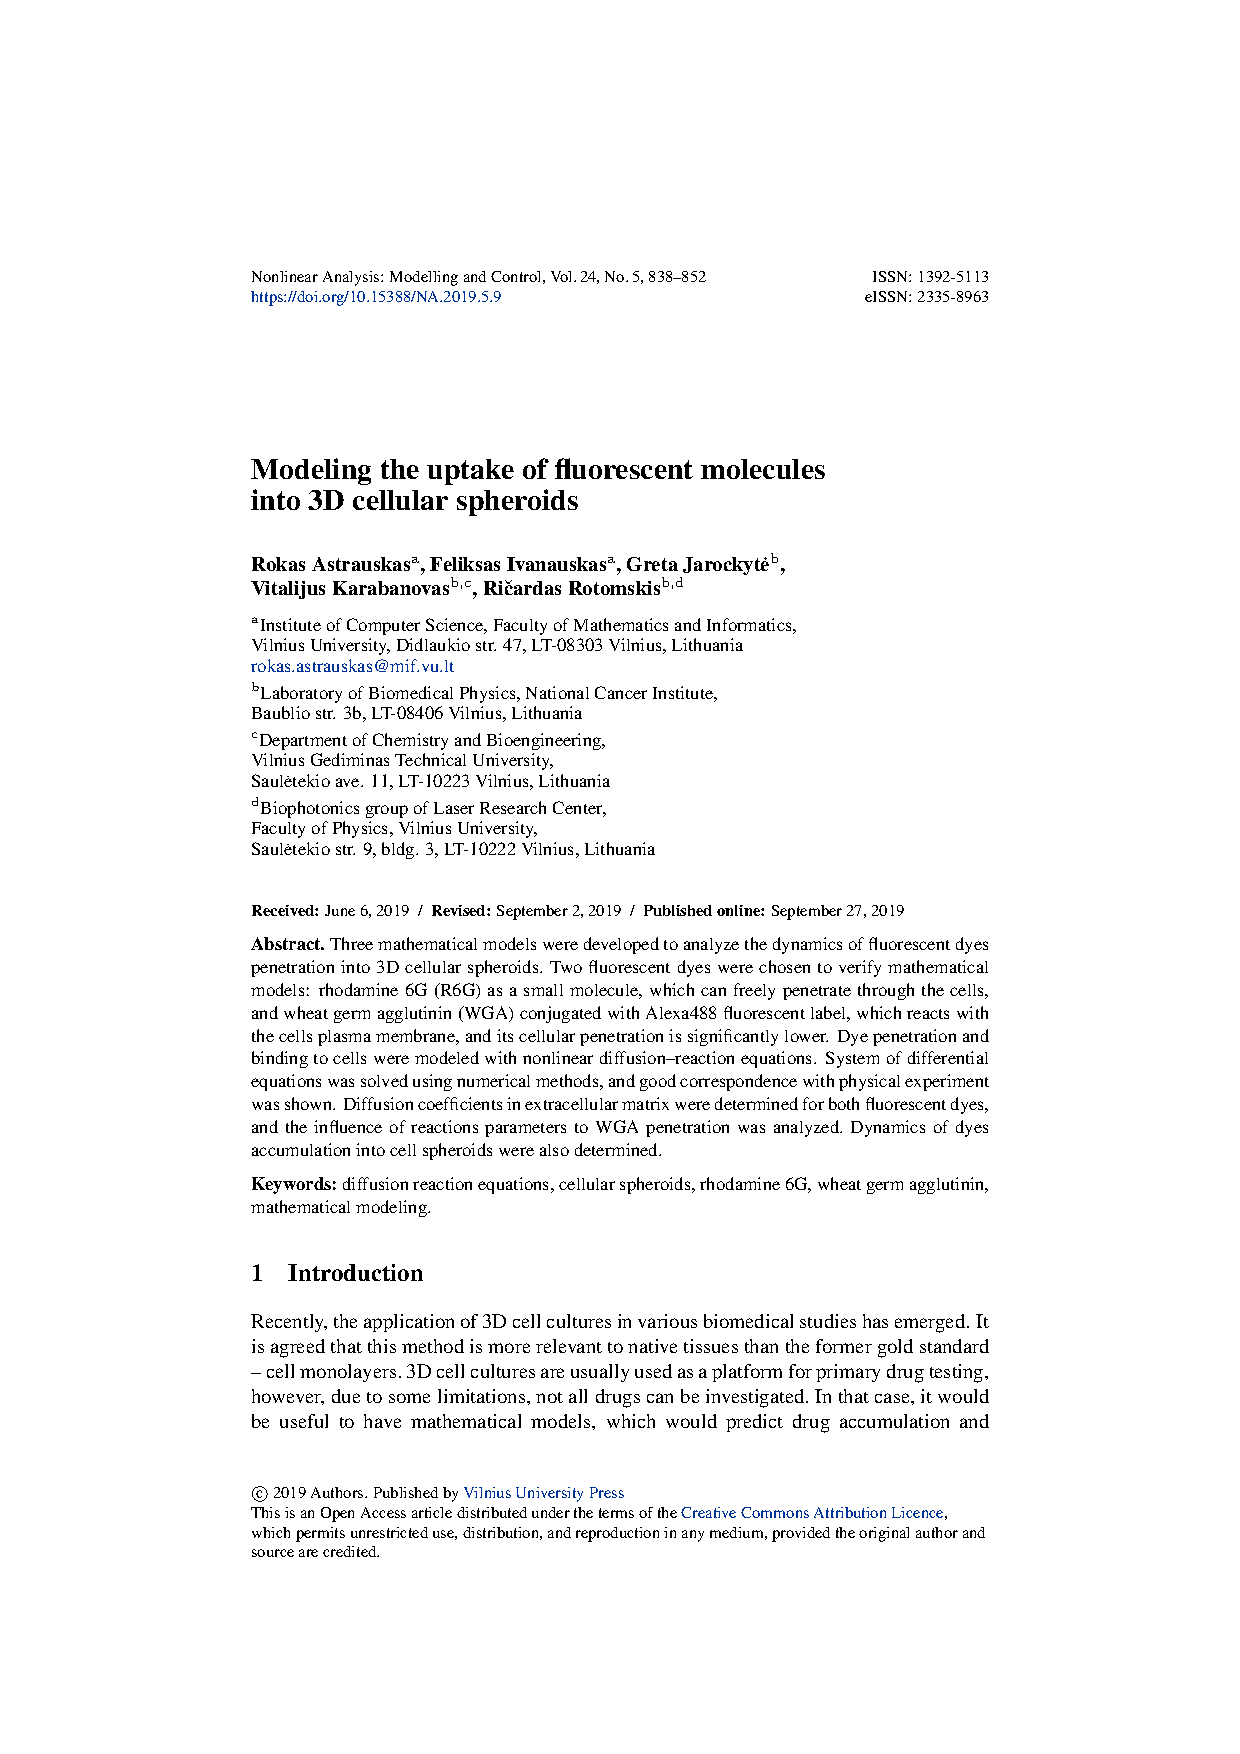
\includepdf[scale=1., pages=-]{publications/Astrauskas2019spheroids.pdf}  

%% Curiculum vitae
%Nors cv reikalavimo nėra, VU doktoranturos skyrius turetų paprašyti pridėti po santraukos gyvenimo aprašymą
%%%%%%%%%%%%%%%%%%%%%%%%%%%%%%%%%%%%%%%%%%%%%%%%%%%%%%%%%%%%%%%%%%%%%%%%%%%%%%%%%%%%%%%%%%%%%%
%% CV is not required in the dissertation body, but it is required in the dissertation summary
%% CV neprašo įdėti į disertacijos turinį, bet prašo įdeti po santraukos
\chapter*{Curriculum Vitae - Gyvenimo aprašymas}
\label{cha:cv}
\addcontentsline{toc}{chapter}{\MakeUppercase{Curriculum Vitae - Gyvenimo aprašymas}}
% \parammarks{Curriculum Vitae}


Vardas Pavardė graduated from ... 

The author's curriculum vitae should be at max one paragraph long.    

%%%%%%%%%%%%%%%%%%%%%%%%%%%%%%%%%%%%%%%%%%%%%%%%%%%%%%%%%%%%%%%%%%%%%%%%%%%%%%%%%%%%%%%%%%%%%%
%% Summary. Note that the main text or summary should be in Lithuanian. Another language preferably is English
%% In this example we use the dissertation language as English and for the summary Lithuanian
% Adding text of Lithuanian summary. 
%Change default parameters for Lithuanian language
\setcounter{section}{0}   %šita automatiškai atnaujina \appendix komanda
\renewcommand*{\thesection}{S.\arabic{section}}
\renewcommand{\thechapter}{S}
\renewcommand{\thefigure}{S.\arabic{figure}}   %raidė S įhardcodinta. Galima švelniau pvz su komanda \thechapter
\setcounter{figure}{0}
\renewcommand{\theequation}{S.\arabic{equation}}
\setcounter{equation}{0}
\renewcommand{\thetable}{S.\arabic{table}}
\setcounter{table}{0}
%jeigu yra dar ko nors, pvz algoritmu, teor ir pan, irgi reikia atnaujinti

\lithuanian   %nustatome lietuviu kalba
\sisetup{output-decimal-marker = {,}}  %lietuviski kableliai ir pan
\sisetup{exponent-product=\ensuremath{\cdot}}


\phantomsection
\chapter*{Summary in Lithuanian / Summary in English}
\label{cha:summary_lt}
\addcontentsline{toc}{chapter}{\MakeUppercase{Summary in Lithuanian - Summary in English}}

% NOTES to the author
% For chapter naming, please use APA style https://titlecapitalize.com/title-case-styles/
    % APA, or American Psychological Style, is one of the most commonly used title case styles in academia. It’s mainly used for research papers in social and behavioral sciences. 
    
    % Its title case rules are also easy enough to remember and follow. Capitalize all major words (nouns, pronouns, verbs, adjectives) in your title, as well as prepositions and conjunction with four or more letters. If your title includes a hyphenated word, capitalize both the initial letters before and after the hyphen. Lastly, the first word after a colon or dash is also capitalized when you’re following the APA style of capitalization for your title or headings.

\chapter*{Introduction / Įvadas}
\label{cha:intro_lt}
\addcontentsline{toc}{chapter}{\MakeUppercase{Introduction / Įvadas}} 

The dissertation must be an original scientific work that substantiates the research problem, defines the \textbf{relevance and purpose of the research work, formulates the goal and objectives of the thesis, indicates the novelty of the scientific work, presents defending statements of the thesis}, reviews the research conducted on the topic of the dissertation in the world (abroad and in Lithuania) and their results, presents the applied research methodology (methods), research results discussed, their reliability and relationship with the data of other researchers, conclusions formulated and other important aspects, in the dissertation's opinion.


\textbf{In Lithuanian}. Disertacija turi būti originalus mokslinis darbas, kuriame pagrindžiama \textbf{tiriamoji problema, apibrėžtas darbo aktualumas, tikslas, suformuluoti sprendžiami uždaviniai, nurodytas mokslinio darbo naujumas, ginami disertacijos teiginiai}, apžvelgti disertacijos tema pasaulyje (užsienyje ir Lietuvoje) atlikti tyrimai ir jų rezultatai, pristatyti taikyta tyrimų metodika (metodai), aptarti tyrimų rezultatai, pagrįstas jų patikimumas ir santykis su kitų tyrėjų duomenimis, suformuluotos išvados ir kiti, disertanto nuomone, svarbūs aspektai.


\phantomsection % Removes warning from hyperref package
\section*{Research Area / Tyrimų sritis}
\addcontentsline{toc}{section}{Research Area / Tyrimų sritis} 

In this section, we recommend briefly introducing the readers to the field of research, which is directly related to the research problem and the aim of the dissertation. Present the current situation in this research area, name the important and relevant research conducted in this area, and present their results. You can attach the research problem section to this section.

\textbf{In Lithuanian}.
Šiame skyrelyje rekomenduojame trumpai skaitytojus supažindinti su tyrimų sritimi, kuri tiesiogiai siejasi su su disertacijos problema ir tikslu. Pristatykite kokia yra dabar situacija šioje srityje, įvardinkite svarbius ir aktualius šioje srityje vykdomus tyrimus ir prisatykite jų rezultatus. Prie šio skyrelio galite prijunti tyrimo problemos skyrelį.

\section*{Research Problem / Tyrimo problema}
\addcontentsline{toc}{section}{Research Problem / Tyrimo problema} 

Definition. A perceived gap between the existing state and a desired state, or a deviation from a norm, standard, or status quo (Bussiness Dictionary\footnote{https://www.bussinessdictionary.com/definition/problem}).

Also:
\begin{itemize}
    \item A problem is a statement, in mathematics or physics, that indicates the need to do something.
    \item The problem is a complex unsolved question. 
    \item A scientific problem can be solved using the steps of the scientific method (e.g. experiments).
\end{itemize}
Before formulating a scientific problem, it is recommended to define the research object and formulate the problem using its concepts.


\textbf{In Lithuanian}. Apibrėžimas. \textbf{Problema} – tai tarpas tarp esamos būsenos ir siekiamos būsenos, arba nukrypimas nuo normos, standarto ar status quo.
Taip pat:
\begin{itemize}
    \item Problema – teiginys, matematikoje ar fizikoje, nurodantis poreikį kažką padaryti.
    \item Problema – sudėtingas neišspręstas klausimas. 
    \item Mokslinė problema – tai klausimas, kuris gali būti atsakytas naudojant mokslinius metodus (pvz., atliekant eksperimentus).
\end{itemize}
Prieš formuojant mokslinę promblemą rekomenduojama apsibrėžti tyrimo objektą ir naudojantis jo sąvokomis suformuluoti problemą.


\section*{Actuality / Darbo aktualumas}
\addcontentsline{toc}{section}{Actuality / Darbo aktualumas} 

The actuality of the research topic is the degree of its importance at the given moment and in this situation for solving these problems, a question or a problem\footnote{\url{https://en.ppt-online.org/424459}}.

In order to show the actuality of the research, you need:
\begin{itemize}
    \item to formulate the research problem
    \item to indicate contradictions found in science or practice that define the research problem
    \item to describe the current situation of the problem with a solution to the problem (is anyone still solving it?)
    \item to describe the importance of research work to society
    \item to generalize and to summarize the best results.
\end{itemize}

\textbf{In Lithuanian}.
Tyrimo temos aktualumas yra sprendžiamos problemos ar klausymo svarbos laipsnis šiuo momentu ir šiuoje situacijoje sprendžiant tyrimo sirties problemas.
Kad parodyti darbo aktualumą reikia:
\begin{itemize}
    \item suformuluoti tyrimo problemą,
    \item nurodyti prieštaravimus kurie aptinkami moksle arba praktikoje, kurie apibrėžia tyrimo problemą, 
    \item apibūdinti esamą problemos situaciją su problemos sprendimu (ar ją kas nors vis dar sprendžia?),
    \item darbo reikšmingumą visuomenei,
    \item apibendrinti geriausius rezultatus.
\end{itemize}


\section*{Research Object / Tyrimo objektas}
\addcontentsline{toc}{section}{Research Object / Tyrimo objektas} 

\textbf{Research object} or research subject is a thing (e.g. algorithm, person, data type) that is used in your research. The research object connects different research contexts: data, analysis tools, hypotheses, experiments, defending statements, and general conclusions. We recommend identifying from 3 to 5 main research concepts and formulating a coherent sentence from them as a research object.
These concepts should also be used in the thesis title and objective. You can read more about how to identify the object of your research on  \url{http://edutechwiki.unige.ch/en/Methodology_tutorial_-_finding_a_research_subject}.

\textbf{In Lithuanian}. \textbf{Tyrimo objektas} (angl. research object, research subject) – daiktas (pvz. algoritmas, asmuo, duomenų tipas), kuris naudojamas detaliame tyrime. Tyrimo objektas susieja skirtingus tyrimo kontekstus: duomenis, analizės įrankius, hipotezes, eksperimentus, ginamuosius teiginius ir išvadas. Rekomenduojame identifikuoti nuo 3 iki 5 pagrindinių tyrimo konceptų ir iš jų suformuluoti nuoseklų sakinį.
Šie konceptai taip pat turėtų būti panaudoti disertacijos pavadinime ir tiksle. Daugiau apie taip kaip identifikuoti savo tyrimo objektą galima paskaityti \url{http://edutechwiki.unige.ch/en/Methodology_tutorial_-_finding_a_research_subject}.



\section*{Research Aim and Objectives / Tyrimo tikslas ir uždaviniai}
\addcontentsline{toc}{section}{Research Aim and Objectives / Tyrimo tikslas ir uždaviniai} 

The goal of science is an action that is performed to solve a defined scientific problem of your research.
The following types of scientific goals are distinguished\footnote{\url{https://opentext.wsu.edu/carriecuttler/chapter/goals-of-science/}}:
\begin{itemize}
    \item The first and most basic goal of science is \textbf{to describe}.
    \item The second goal of science is \textbf{to predict}.
    \item The third and ultimate goal of science is \textbf{to explain}.
\end{itemize}
When defining the main goal of the dissertation, it is recommended to think about what you managed \textbf{to create} in your dissertation. Thus, defining the goal will make it easier for you to describe the novelty and originality of the research work. 
If your research aims to create a solution, a tool, or an algorithm, it will also be related to scientific aims: to describe, predict, or explain.

For the aim of research, the only requirement is \textbf{it must be measurable}.

Research objectives are smaller actions required to achieve the aim. They must also be measurable. 
The research objective must be relevant, related to the aim, feasible, logical, measurable, and unambiguous.
When executing the objective, we aim to find answers to questions or test research hypotheses.

It is recommended that each objective relates to at least one defending statement and at least one thesis general conclusion. This way you will achieve consistency and integrity of your work. It is recommended that the number of research tasks should be between 3 and 5.

\textbf{In Lithuanian}. 
Mokslo tikslas tai veiksmas kuris atliekamas norint išspręsti apibrėžtą savo tyrimo mokslinę problemą. 
Yra išskiriami šie mokslo tikslų tipai:
\begin{itemize}
    \item Pirmas ir bazinis mokslo tikslas – „\textbf{Aprašyti}/apibūdinti/apibrėžti“ (angl. to describe).
    \item Antras mokslo tikslas – „\textbf{Prognozuoti}“ (angl. to predict“).
    \item Trečiasis ir pagrindinis mokslo tikslas „\textbf{Paaiškinti}/Suprasti“ (angl. to explain/understand).
\end{itemize}

Konstruojant pagrindinį disertacijos tiklsą rekomenduojama pagalvoti, o ką jūsų darbe pavyko  \textbf{sukurti}, taip apibrėžiant tikslą jums lengviau bus aprašyti darbo naujumą ir orgiginalumą. Darbo tikslas, kaip sukurtas sprendimas, įrankis ar algoritmas siesis ir mokslo tikslais: aprašyti, prognozuoti ar paaiškinti.

Tyrimo tikslui, keliamas vienintelis reikalavimas - \textbf{jis turi būti pamatuojamas}.

Tyrimo uždaviniai tai mažesni veiksmai reikalingi užsibrėžtam tikslui pasiekti. Jie taip pat turi būti  pamatuojami. 
Mokslinis uždavinys turi būti, aktualus, susijęs su tikslu, įvykdomas, logiškas, pamatuojamas, nedviprasmiškas.
Spręsdami uždaviniais mes siekiame surasti atsakymus į klausimus arba patikrinti tyrimo hipotezes.

Rekomenduojama, kad kiekvienas uždavinys sietųsi su bent vienu ginamuoju teiginiu ir su bent su viena disertacijos išvada. Taip pasieksite darbo nuoseklumo ir vientisumo. Rekomenduojama, kad tyrimo uždavinių kiekis būtų nuo  3 iki 5.

\section*{Research Methods / Tyrimo metodai}
\addcontentsline{toc}{section}{Research Methods / Tyrimo metodai} 

Research methods are specific procedures for collecting and analyzing data. Developing your research methods is an integral part of your research design. For more about available research methods, please read on \url{https://www.scribbr.com/category/methodology/}.

\textbf{In Lithuanian}. 
Tyrimo metodai – tai specifinės duomenų rinkimo ir analizės procedūros. Tyrimo metodų kūrimas yra neatsiejama jūsų tyrimo plano dalis. Daugiau tyrimo metodus, skaitykite \url{https://www.scribbr.com/category/methodology/}.


\section*{Scientific Novelty / Mokslinis darbo naujumas} %Scientific Contribution of the Research
\addcontentsline{toc}{section}{Scientific Novelty / Mokslinis naujumas} 

This is one of the main requirements for the dissertation. This means that the dissertation must have a solution to a new scientific problem or a new development that allows expanding the existing boundaries of knowledge in a certain branch of science.

A job is new if:
\begin{itemize}
 \item it is a new interesting question (problem) or topic,
 \item it is a little researched question (problem) or not studied in depth.
\end{itemize}

Novelty can be associated with the reuse of old ideas in new conditions, new fields of science, or practice.

The novelty of the work can be achieved by the following methods:
\begin{itemize}
 \item Introduction of new previously unused sources (methods, laws, theorems) into the existing field of science and their subsequent analysis.
 \item New interpretation of existing and known sources and addition or correction of existing knowledge.
 \item Researching little-understood or analyzed sources of old information and their aspects.
\end{itemize}


\textbf{In Lithuanian}. Tai vienas iš pagrindinių reikalavimui disertacijos temai. Tai reiškia kad darbas turi turėti sprendimą naujai mokslinei problemai, arba nauja plėtra kuri leidžia praplėsti egzistuojančias tam tikros mokslo šakos žinių ribas.
Darbas yra naujas, jeigu:
\begin{itemize}
    \item tai naujas įdomus klausimas (problema) ar tema,
    \item tai mažai tyrinėtas klausimas (problema) ar netyrinėtas giliai.
\end{itemize}

Naujumas gali būti susietas su senų idėjų pakartotiniame panaudojimu naujose sąlygose, naujose mokslo ar praktikos srityse.

Darbo naujumas gali būti pasiektas šiais metodais:
\begin{itemize}
    \item Naujų ankščiau nenaudotų šaltinių (metodai, dėsniai, teoremos) įvedimas į esamą mokslo sritį ir vėlesnė jų analizė.
    \item Nauja esamų ir žinomų šaltinių interpretacija ir esamų žinių papildymas ar pataisymas.
    \item Tyrinėjimas mažai suvoktus ar išanalizuotus senos informacijos šaltinius, jų aspektus.
\end{itemize}



\section*{Practical Significance / Praktinė darbo vertė}  %Gali būti impact, kuris žodis geresnis? ar Practical Value of the Research
\addcontentsline{toc}{section}{Practical Significance / Praktinė darbo vertė} 

In this section, discuss the practical benefits of the results of this dissertation work. Describe where and how they were, are, or can be applied in practice. Or indicate how they contribute to solving practical problems.

\textbf{In Lithuanian}. 
Šiame skyrelyje pakalbėkite apie šio disertacijos darbo rezultatų praktinę naudą. Aprašykite kur ir kaip jie buvo, yra ar gali būti pritaikyti praktikoje. Arba nurodykite kaip jie prisideda prie praktinių problemų sprendimo.

\section*{Statements to be Defended / Ginamieji teiginiai}
\addcontentsline{toc}{section}{Statements to be Defended / Ginamieji teiginiai}

According to the recommendations set by the Lithuanian Science Council for the structure of the dissertation, the introduction must contain defending statements, which must also be reflected in the conclusions.
There are no more detailed requirements defining what the defending statements are or how many of them there should be - so it is enough to remind you of the previously mentioned advice to read theses defended in a specific discipline and participate in their defenses.

The answer to the question of what are defending statements can be found in another way - by clarifying the concept of "defending statement".
\begin{itemize}
    \item First, it must be a statement (not a question).
    \item Second, it must be a statement that is defended in the thesis, i.e. a statement that is not self-evident and requires justification. 
\end{itemize}
A defending statement is just the equivalent of a thesis with a different name - it states what and how it is intended to be proved.
In many cases, the equivalent of a defending statement can be a hypothesis - in the dissertation, we test assumptions about an expected relationship.

The recommended number of defending statements is from 3 to 5. They must also be related to the research objectives and conclusions.

\textbf{In Lithuanian}. 
Pagal  Lietuvos  mokslo  tarybos  nustatytas  rekomendacijas  disertacijos struktūrai, įvade turi būti suformuluoti ginamieji teiginiai, kurie taip pat jie turi atsispindėti išvadose. 
Detalesnių reikalavimų, apibrėžiančių, kas  yra  ginamieji  teiginiai  ar kiek jų  turėtų būti,  nėra nustatyta – todėl telieka priminti jau anksčiau minėtą patarimą skaityti konkrečioje disciplinoje gintas disertacijas ir dalyvauti jų gynimuose (Doktorantūros studijų kokybės valdymas, metodinė medžiaga doktorantų vadovams ir doktorantams, VU, 2013 m.\footnote{\url{https://www.mii.vu.lt/files/doc/lt/doktorantura/dokumentu_sablonai/doktoranturos_studiju_kokybes_valdymas_metodine_medziaga_doktorantu_vadovams_ir_doktorantams1.pdf}
}).

Atsakymo į klausimą, kas yra ginamieji teiginiai, galima ieškoti ir kitu keliu – išsiaiškinant „ginamojo teiginio“ sąvoką. 
\begin{itemize}
    \item Pirma, tai turi būti teiginys (o ne klausimas). 
    \item Antra, tai turi būti teiginys, kuris disertacijoje yra ginamas, t.y. teiginys, kuris nėra savaime akivaizdus ir kurį reikia pagrįsti. 
\end{itemize}
Ginamasis teiginys yra tik kitaip įvardintas tezės ekvivalentas – juo įvardijama, kas ir kaip ketinama įrodinėti. 
Ginamojo teiginio ekvivalentu daugeliu atveju gali būti hipotezės – disertacijoje tikrinami spėjimai apie numatomą priežastinį ryšį.

Rekomenduojamas ginamųjų teiginių kiekis nuo  3 iki 5. Ir jie turi sietis su turimo uždaviniais ir darbo išvadomis.


\section*{Approbation and Publications of the Research/ Tyrimo aprobavimas ir publikavimas} %Darbo rezultatų aprobavimas
\addcontentsline{toc}{section}{Approbation and Publications of the Research/ Tyrimo aprobavimas ir publikavimas} 

Your dissertation must meet the formal requirements, i.e., the results presented in the dissertation had to be published in at least two journals indexed in the Web Of Science database and discussed at two international conferences.
In this section, a list of publications published in the Web Of Science database (same as \nameref{cha:publications}) and list of all other publication should be presented. Additionally, provide a list of all scientific events where you have given presentations on the topic of the dissertation.

\textbf{In Lithuanian}. 
Jūsų disertacija turi tenkinti formalius reikalavimus, t.y. disertacijoje pristatomi rezultatai turėjo būti išspausdinti bent dviejuose žurnaluose indeksuojamuose Web Of Science duomenų bazėje, ir aptarti bend dvejose tarptautinėse konferencijose.
Šiame skyrelyje pateiktite sąrašą visų disetacijos tema išspaudintų darbų iš jų išskiriant publikacijas pakslebtas Web Of Science duomenų bazėje (tas pats kaip ir skyriuje \nameref{cha:publications}). Papidlomai pateikite sąrašą visų mokslinių renginių kuriuose skaitėte pranešimus disertacijos tema.


\section*{Outline of the Thesis/ Disertacijos strukūra}
\addcontentsline{toc}{section}{Outline of the Thesis/ Disertacijos strukūra} 

In this section, present the main sections of the thesis and the overall size of the thesis.

This doctoral thesis consists of an introduction, ... chapters, conclusions, and a summary in the Lithuanian language. The introduction section provides an introduction to the research and an overview of the dissertation. The first chapter is ...

... bibliographic references are included at the end of the thesis. The disertation consist of ... pages, ... figures and ... tables.


\textbf{In Lithuanian}. 

Šiame skyrelyje pristatykite pagdindinius disertacijos skyrius ir bendrą disertacijos apimtį.



\textbf{Note} Please translate all parts of the introduction to Lithuanian and put them into the \verb|chapter_intro_lt.tex| file.
\textbf{In Lithuanian}. \textbf{Pastaba}Angliško ir lietuviško įvado turinys turi būti identiškas turinio prasme. Išverstą tekstą patalpinkite \verb|chapter_intro_lt.tex| failą.

% !TEX encoding = UTF-8 Unicode

\pagestyle{plain}

%\lithuanian

\phantomsection % Removes warning form hyperref package
\section*{Tyrimų sritis}
\addcontentsline{toc}{section}{Research Area / Tyrimų sritis}

Pasitelkus kompiuterinį modeliavimą disertacijoje tiriamos su\-dė\-tin\-gos cheminės ir biofizikinės sistemos, kurios yra aprašomos dalinių išvestinių lygtimis (DIL) su netiesinėmis kraštinėmis sąlygomis ir DIL sudėtingos geometrijos (nestačiakampėse) srityse. Šios DIL sprendžiamos baigtinių skirtumų metodu ir kitais skaitiniais algoritmais. 

%Disertacijoje tiriamos sudėtingos cheminės ir biofizikinės sistemos naudojant kompiuterinį modeliavimą. Šios sistemos yra aprašomos dalinių išvestinių lygtimis (DIL) su netiesinėmis kraštinėmis sąlygomis ir DIL sudėtingos geometrijos (nestačiakampėse) srityse. Šios DIL sprendžiamos baigtinių skirtumų metodu ir kitais skaitiniais algoritmais.  
%The study is focused on computer modelling of complex chemical and biophysical systems, which are described by partial differential equations (PDEs) with nonlinear boundary conditions and PDEs in various complex (non-rectangular) domains. Differential problems are solved using numerical methods
%Tyrimas skirtas išspręsti dalinių išvestinių lygtims (DIL) su netiesinėmis kraštinėmis sąlygomis sistemas ir išspręsti DIL sudėtingos geometrijos (nestačiakampėse) srityse, naudojant skaitinius metodus.

DIL sprendimo su netiesinėmis kraštinėmis sąlygomis problemos kyla dėl cheminių ir biologinių procesų matematinio modeliavimo. 
Tyrimai nestačiakampėse srityse yra aktualūs dėl poreikio įvertinti matavimo prietaisų paklaidas, atsirandančias dėl geometrijos nukrypimo nuo standarto.
%Tyrimai nestačiakampėse srityse yra aktualūs dėl poreikio modeliuoti nukrypimus nuo normos įrangoje, naudojamoje cheminiams ir biologiniams eksperimentams. 
DIL netiesinės sistemos yra pritaikytos tyrinėti chemoterapinių vaistų patekimą į audinius.





\section*{Tikslas}
\addcontentsline{toc}{section}{Tikslas} 
...





%--------------- SECM Redox reakciju skyrius ---------------------------------
%--------------------------------------------------------------------------

\section{SECM modeliavimas oksidacijos-redukcijos konkurencijos režime}
\label{sec:santr_reakc}



\subsection{Matematinis modelis}

Dėl simetrijos aplink centrinę elektrodo ašį modelis užrašomas cilindrinėse koordinatėse. Cilindro formos srityje atliekami SECM matavimai yra pakeisti į 2D sritį \ref{fig:santr_Domain} pav.


\begin{figure}[ht!]
\centering
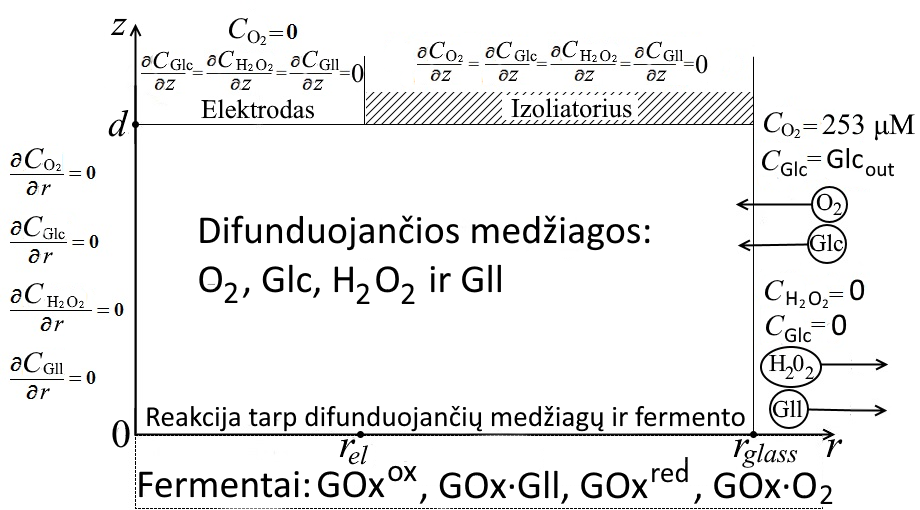
\includegraphics[width=0.8\linewidth]{summary/Model_domainLT.png}
\caption{Modeliavimo srities schema. Pavaizduotos $8$ modeliuotos medžiagos - $4$ difunduojantys reagentai bei $4$ fermento GOx formos, kraštinės sąlygos 4-ioms difunduojančioms medžiagoms ir išorinis srautas.}
\label{fig:santr_Domain}
\end{figure}

Difuzijos procesai išreiškiami antruoju Fiko dėsniu:
\begin{equation}
  \begin{aligned}\label{eq:santr_eq1}
  \frac{\partial C_{O_2}}{\partial t} &= D_{O_2}\,\Delta C_{O_2},\\
  \frac{\partial C_{Glc}}{\partial t} &= D_{Glc}\,\Delta C_{Glc},\\
  \frac{\partial C_{H_2 O_2}}{\partial t} &= D_{H_2 O_2} \,\Delta C_{H_2 O_2},\\
  \frac{\partial C_{Gll}}{\partial t} &= D_{Gll}\,\Delta C_{Gll},  \quad 0<t\leq T,\; 0<z<d,\; 0<r<r_{glass}.
  \end{aligned}
\end{equation}
Šiose lygtyse:
\begin{itemize}
  \item[] $C_{O_2}$, $C_{Glc}$, $C_{H_2 O_2}$ ir $C_{Gll}$ yra atitinkamų difunduojančių re\-a\-gen\-tų koncentracijos, kurios išreiškiamos kaip laiko $t$, er\-dvi\-nių ko\-or\-di\-na\-čių $z$ ir $r$ funkcijos. 
  \item[] $D_{O_2}$, $D_{Glc}$, $D_{H_2 O_2}$ ir $D_{Gll}$ yra difuzijos koeficientai.
  \item[] $d$ yra atstumas tarp fermentu modifikuoto paviršiaus ir elektrodo. Skaitinio eksperimento metu $d$ keičiamas nuo $\SI{1}{\um}$ iki $\SI{120}{\um}$. Tai atitinka elektrodo stumdymą aukštyn ir žemyn cheminio eksperimento metu.
  \item[] $r_{glass} = \SI{80}{\um}$ yra izoliuotos srities spindulys.
  \item[] $T$ yra skaičiavimo eksperimento trukmė, matuojama sekundėmis.
  \item[] Laplaso operatorius $\Delta$ cilindrinėse koordinatėse su centrine simetrija yra
  \begin{equation*}
  \Delta C = \frac{1}{r}\frac{\partial C }{\partial r} \left( r\frac{\partial C }{\partial r} \right) + \frac{\partial^{2} C}{\partial z^{2}}.
  \end{equation*}
\end{itemize}


\chapter*{General conclusions / Bendrosios išvados }
\label{cha:concl_lt}
\addcontentsline{toc}{chapter}{\MakeUppercase{General conclusions / Bendrosios išvados}} 

It is recommended that these conclusions relate directly to the objectives and defending statements of the thesis. 
The conclusions should accurately reflect the results obtained in the dissertation work.
The recommended number of conclusions is 3-5.

\textbf{Note}. Please do a direct translation of the conclusion to Lithuanian language and put them to the \verb|chapter_concl_lt.tex|.


\textbf{In Lithuanian} Šiame skyriuje pateikite sąrašą pagrindinių disertacijos išvadų. Rekomenduojama, kad šios išvados tiesiogiai sietųsi su darbo uždaviniais ir ginamaisiais teiginiais. Išvadose turėtų tiksliai atsispindėti rezultatai gauti disertacijos darbe. 
Rekomenduojamas išvadų kiekis 3-5.

\textbf{Pataba}.Jeigu disertaciją rašote lietuviškai, tuomet išvadas išverskite į anglų kalbą ir pateikite \verb|chapter_concl.tex| faile, kuris būtų naudojamas angliškoje disertacijos santraukoje.
Jeigu disertaciją rašote angliškai, tuomet išverskite į lietuvių kalbą ir pateikite \verb|chapter_concl_lt.tex| faile.

\british  %griztame prie anglu kalbos

\backmatter

\restoreParagraph
%%%%%%%%%%%%%%%%%%%%%%%%%%%%%%%%%%%%%%%%%%%%%%%%%%%%%%%%%%%%%%%%%%%%%%%%%%%%%%%%%%%%%%%%%%%%%%
%% Indexes. Optional
% [file: index.tex, started: 25-Aug-2005]
%
% PhD Thesis - top level LaTeX source file.
%
% DESCRIPTION
%   This file includes Index chapter of the PhD Thesis. 
%   USe command \index{keyword} to add "keyword" to the index
%
% CHANGES
%   2005.08.25  *  Started.
%   2008.03.18  *  Adapted to IZ.
%   2024.08.30  *  Fixed to fit VU dissertation template
% \chapter{Index}
% \label{chapter:Index}

\addtocontents{toc}{\protect\enlargethispage{2\baselineskip}}
\phantomsection
% \addcontentsline{toc}{chapter}{\numberline{}Index} % \numberline{} atitraukia į šalį
\addcontentsline{toc}{chapter}{\MakeUppercase{Index}}

%To add something to index please use command \index{keyword}
%Show index items in two-column style sorted by name
{\raggedright
    \printindex
}
  %indeksas - nuorodos į puslapius, kur panaudota kokia svarbi savoka. Nereikalinga	

%%%%%%%%%%%%%%%%%%%%%%%%%%%%%%%%%%%%%%%%%%%%%%%%%%%%%%%%%%%%%%%%%%%%%%%%%%%%%%%%%%%%%%%%%%%%%%
%% Finalize the document by adding publishing information
%% Pačioje pabaigoje pridedama spausdinimo informacija (pvz., pavadinimas ir leidykla)
\pagestyle{empty}

\iffalse   
\begin{center}   %Jeigu truktu puslapiu. Leidykla prasys kad dalintusi is 4
NOTES
\end{center}
\newpage
\fi

\cleardoublepage



\vspace{165mm}

\begin{flushleft}
Rokas Astrauskas
	
Computer Modelling of Reaction-Diffusion Processes\\ 
in Scanning Electrochemical Microscopy and in Cell Spheroids

Doctoral Dissertation\\
Natural Sciences\\
Informatics (N 009)\\
Thesis Editor: ...


\vspace{3cm}

Reakcijos-difuzijos procesų kompiuterinis modeliavimas\\
skenuojančioje mikroskopijoje ir ląstelių sferoiduose

Daktaro disertacija\\
Gamtos mokslai\\
Informatika (N 009)\\
Santraukos redaktorė: ...


\end{flushleft}




\vspace{165mm}

{
	\vspace*{\fill}
	
	\centering
Vilnius University Press\\
9 Saulėtekio Ave., Building III, LT-10222 Vilnius\\
Email: info@leidykla.vu.lt, www.leidykla.vu.lt\\
Print run of ... copies\\
}
  

\end{document}